\section{Impact of Warmup Steps}
\label{apx:warmup}
We investigate the impact of LR warmup steps on loss curves. Specifically, different values of warmup steps are experimented. As shown in Fig.~\ref{fig:warmup_diff}, we find that a warmup step value of 500 accelerates convergence and achieves the lowest validation loss compared to 100 or no warmup.
This finding is aligned with previous works~\citet{warmup-evidence,kosson2024analyzing}. 

Based on these findings, 
we use 500 warmup steps in our main experiments when training models from scratch.
Note that LR warmup when training a randomly initialized model is different from LR re-warmup in continual training. In fact, the re-warmup process can be seen as a special types of LRS where $S_2<0$ in our equation.



\begin{figure}[htbp]
    \centering
    \begin{subfigure}[b]{0.6\textwidth}
        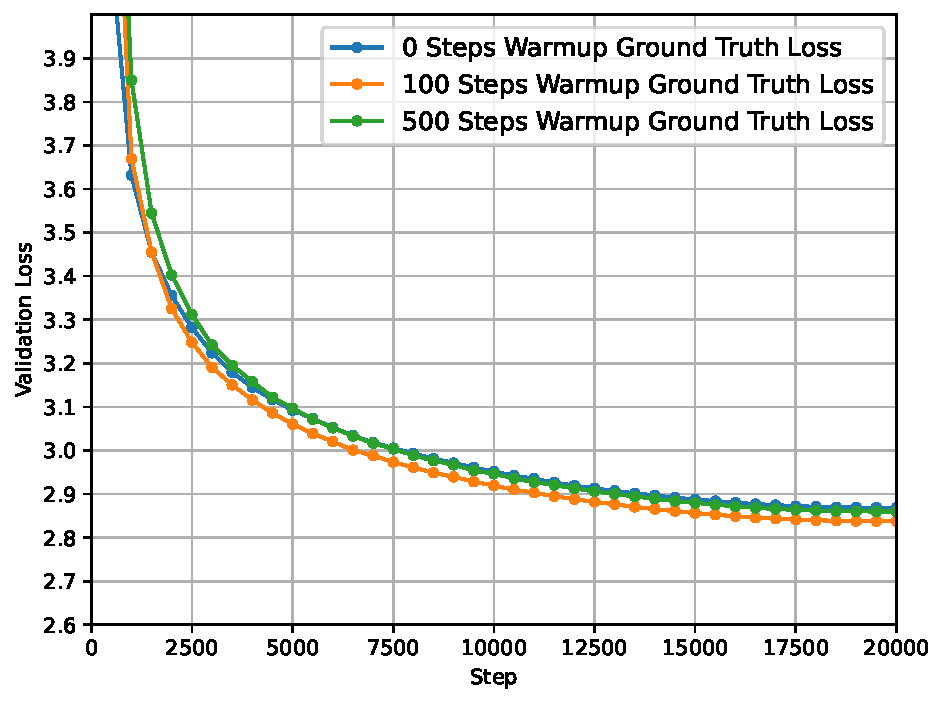
\includegraphics[width=\textwidth]{images/warmup_diff.pdf}
    \end{subfigure}
    \caption{Validation loss curves corresponding to different warmup steps. We use cosine LRS with 20K total steps.}
\label{fig:warmup_diff}
\end{figure}

\section{Experimental Setups}
\label{apx:exp-sets}
In this work, we use multiple experimental setups to validate the effectiveness of our equation across a variety of conditions. For clarity, we summarize all experimental setups in Table~\ref{tab:exp-sets}. The majority of our experiments use Setting A. Additionally we also successfully fit our equation to the loss curves of BLOOM \citep{workshop2022bloom} and OLMo \citep{groeneveld2024olmo}. The experimental settings used to produce these loss curves are significantly different from ours. Please refer to their papers for details on their specific experimental setups.

\begin{table}[p]
\begin{center}
\caption{Experimental settings adopted in this work. Model size denotes the number of non-embedding parameters. Our datasets include Fineweb~\citep{penedo2024fineweb} and RedPajama-CC~\citep{together2023redpajama}. 
* denotes pre-training multilingual datasets including mixture of sources such as common crawls, books, arxiv, code, etc.
We use AdamW Optimizer~\citep{adam-optim,loshchilov2017decoupled}, denoted as AO.
Most experiments adopt Llama-3's tokenizer~\citep{dubey2024llama}.
Ext Llama-2's is extended from Llama-2's tokenizer ~\citep{touvron2023llama} by adding vocabulary.}
\label{tab:exp-sets}
\begin{tabular}{llll}
\toprule
\textbf{Setups} & \textbf{Setting A (main)} & \textbf{Setting B} & \textbf{Setting C}
\\
\midrule
\textbf{Model Size} & $594$M & $293$M & multiple \\
\textbf{Train Dataset} & Fineweb & Finweb & Mixture-train* \\ 
\textbf{Val Dataset} & RedPajama-CC & RedPajama-CC & Mixture-valid* \\
\textbf{Total Steps} & $60$K & $120$K & $143$K \\
\textbf{Maximal LR} & $2\times10^{-4}$ & $2\times10^{-4}$ & $1.381\times10^{-3}$ \\
\textbf{Warmup Steps} & $500$ & $100$ & $500$ \\
\textbf{Batch Size (tokens) } & $4$M & $2$M & $4$M \\
\textbf{Sequence Length} & $4096$ & $4096$ & $4096$ \\
\textbf{Tokenizer} & Llama-3's & Llama-3's & Ext Llama-2's \\
\textbf{$\beta_1$,$\beta_2$ in AO} & $0.9$, $0.9$5 &  $0.9$, $0.95$ & $0.9$, $0.95$\\
\textbf{Weight Decay}  & $0.1$ & $0.1$ & $0.1$\\
\textbf{Gradient Clip}  & $1.0$ & $1.0$ & $1.0$\\
\bottomrule  % WARNING: it cannot change to top/mid rule for unrecognized fatal bug
\toprule
\textbf{Setups} & \textbf{Setting D (MoE)} & \textbf{Setting E (1.4T tokens)} &  \\
\midrule 
\textbf{Model Size} & $8\times106$M & $1704$M &  \\
\textbf{Train Dataset} & Fineweb & Mixture-train* &  \\ 
\textbf{Val Dataset} & RedPajama-CC & Mixture-valid* &  \\
\textbf{Total Steps} & $60$K & $350$K & \\
\textbf{Maximal LR} & $2\times10^{-4}$ & $6\times10^{-4}$ & \\
\textbf{Warmup Steps} & $500$ & $1000$ & \\
\textbf{Batch Size (tokens) } & $4$M & $4$M & \\
\textbf{Sequence Length} & $4096$ & $8192$ & \\
\textbf{Tokenizer} & Llama-3's & Llama-3's &  \\
\textbf{$\beta_1$,$\beta_2$ in AO} & $0.9$, $0.9$5 &  $0.9$, $0.95$ & \\
\textbf{Top-$k$ Experts} & $2$ & - &  \\
\textbf{Auxiliary Loss} & $0.01$ & - &  \\
\textbf{Weight Decay}  & $0.1$ & $0.1$ & \\
\textbf{Gradient Clip}  & $1.0$ & $1.0$ & \\
\bottomrule
\end{tabular}
\end{center}
\end{table}

\section{Results on Extensive Experiments Setups}
\subsection{Another Set of Training Hyper-parameters}
\label{apx:exp-2}
Fig.~\ref{fig:fit} and Fig.~\ref{fig:prediction} show that our equation can work very well on our main experimental setup detailed in Table~\ref{tab:exp-sets}.
To validate the effectiveness of our scaling law formulation on different experimental settings, we report the results on Setting $B$ (see Table~\ref{tab:exp-sets}). The fitting results are shown in Fig.~\ref{fig:fit_12w}, and the prediction results are shown in Fig.~\ref{fig:predict_12w}. The results suggest that our scaling law with LR annealing works well across different experimental setups.

\newpage

\begin{figure}[tbp]
    \centering
    \begin{subfigure}[b]{0.32\textwidth}
        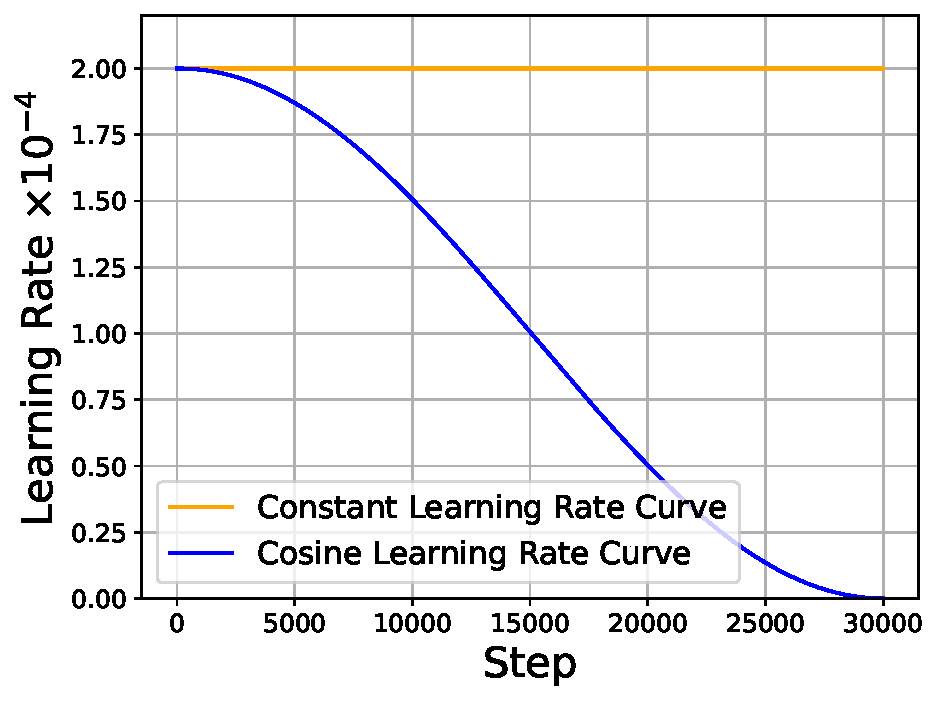
\includegraphics[width=\textwidth]{images/plot_newxy/12w_lr_fit.pdf}
        \caption{Learning rate.}
    \end{subfigure}
    \hfill
    \begin{subfigure}[b]{0.32\textwidth}
        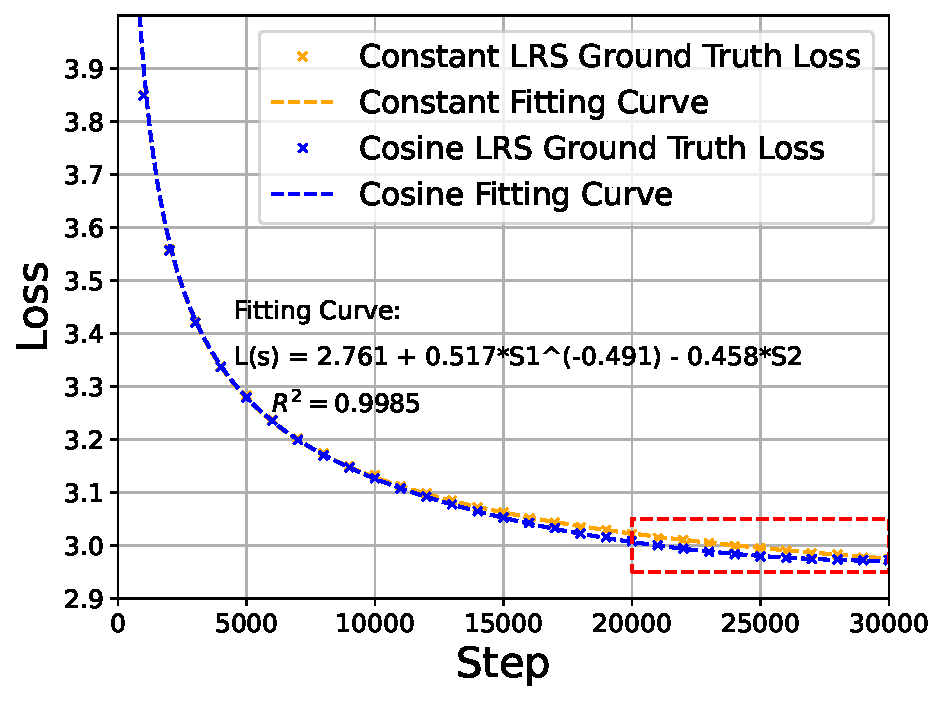
\includegraphics[width=\textwidth]{images/plot_newxy/12w_predict_fit_zoomout.pdf}
        \caption{Zoomed-out loss fitting.}
    \end{subfigure}
    \hfill
    \begin{subfigure}[b]{0.32\textwidth}
        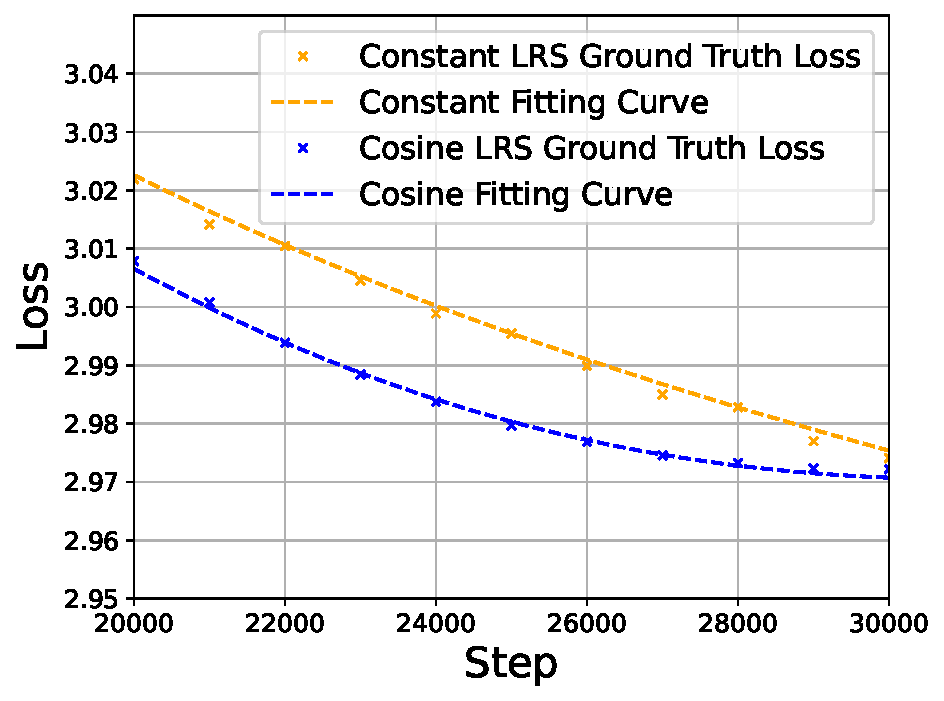
\includegraphics[width=\textwidth]{images/plot_newxy/12w_predict_fit_zoomin.pdf}
        \caption{Zoomed-in loss fitting.}
    \end{subfigure}
    \caption{Using Eq.\ref{eq:scaling} to \textbf{fit} full loss curves yield by cosine and constant LRS. Total steps=30K, $\eta_{min}=2\times 10 ^{-4}$, $\eta_{min}=0$. We omit the warmup steps in the figure. The fitted equation is $L = 2.761 + 0.517\cdot S_1^{-0.491} - 0.458\cdot S_2$. Refer to setting B in Table~\ref{tab:exp-sets} for detailed experimental setups.}
\label{fig:fit_12w}
\end{figure}


\begin{figure}[tbp]
    \centering
    
    \begin{subfigure}[b]{\textwidth}
        \centering
        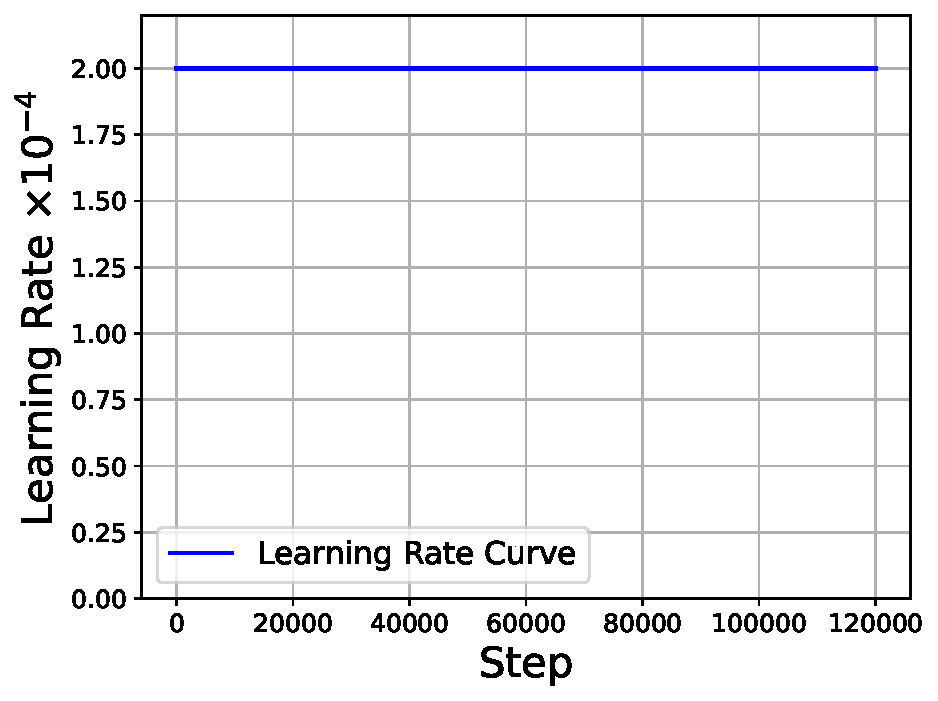
\includegraphics[width=0.32\textwidth]{images/plot_newxy/12w_lr_constant.pdf}
        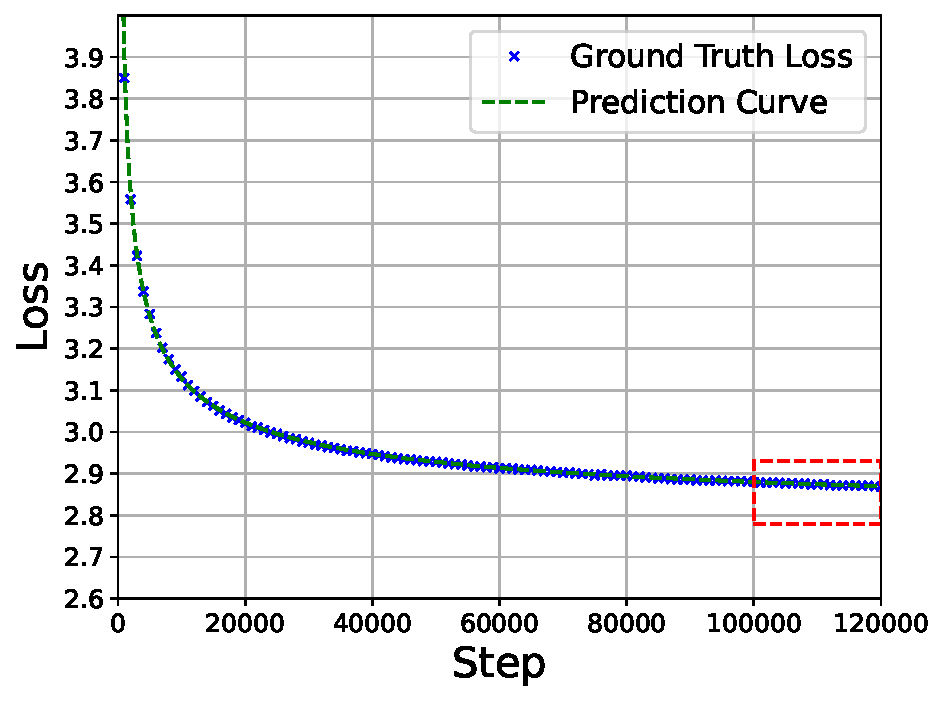
\includegraphics[width=0.32\textwidth]{images/plot_newxy/12w_predict_constant_zoomout.pdf}
        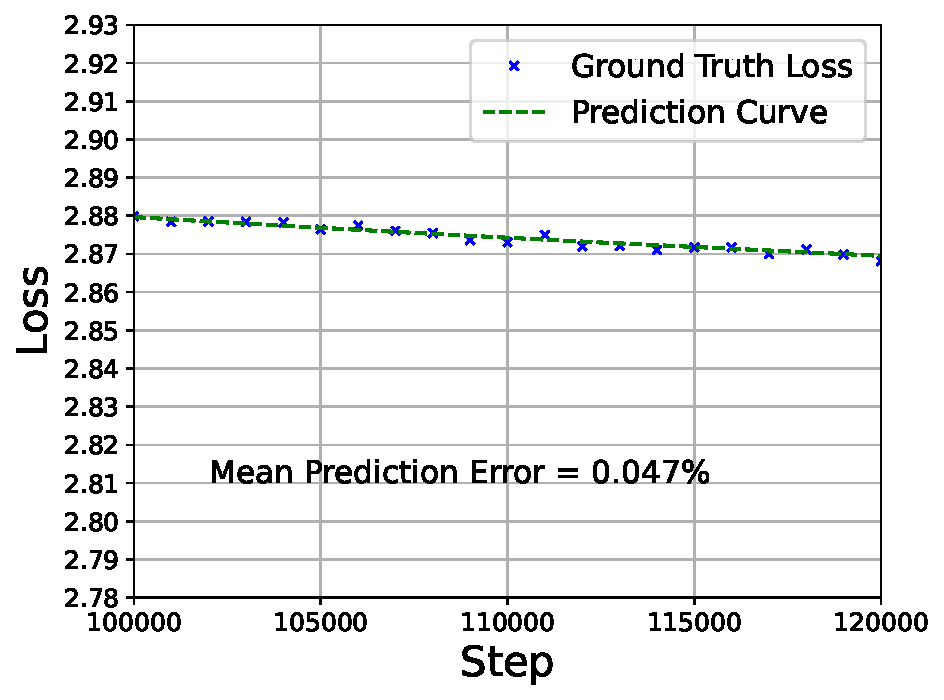
\includegraphics[width=0.32\textwidth]{images/plot_newxy/12w_predict_constant_zoomin.pdf}
        \caption{Full curve prediction of constant LRS.}
        \label{fig:prediction-12w-constant}
    \end{subfigure}

    \begin{subfigure}[b]{\textwidth}
        \centering
        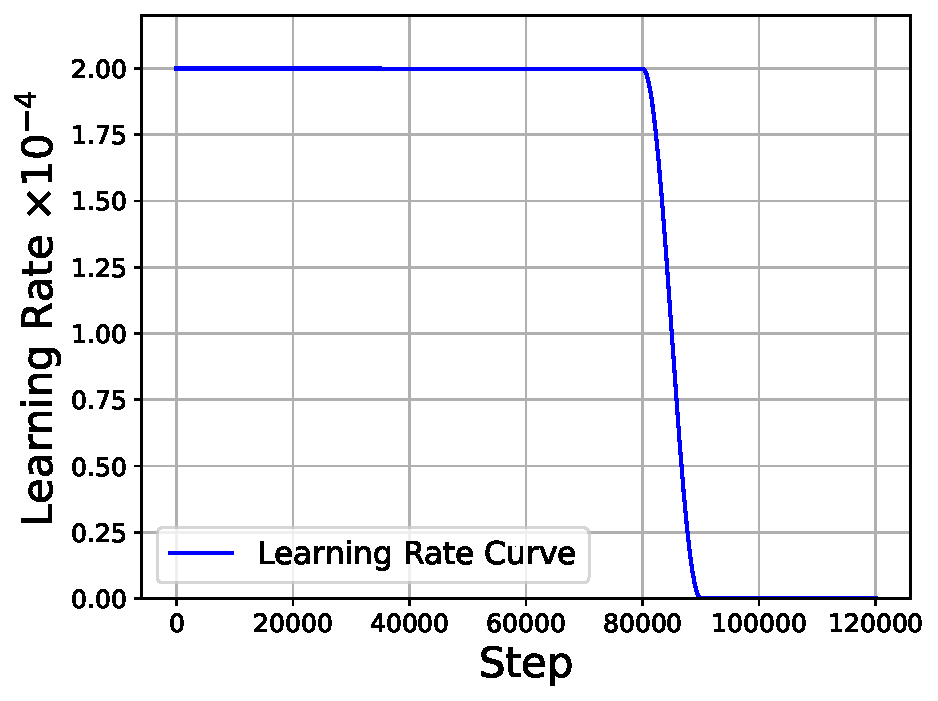
\includegraphics[width=0.32\textwidth]{images/plot_newxy/12w_lr_wsd.pdf}
        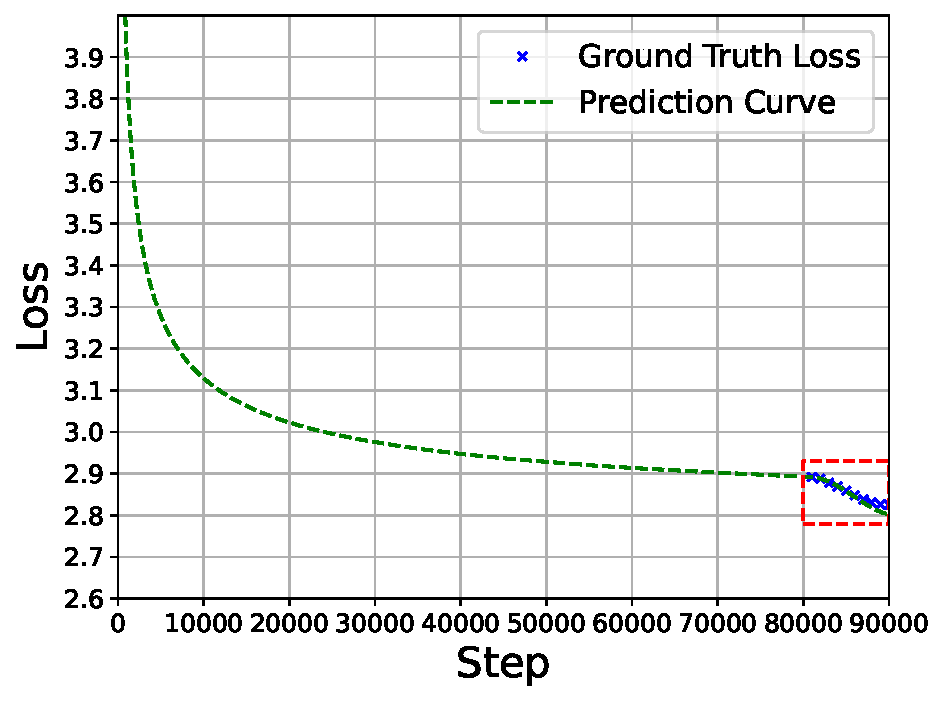
\includegraphics[width=0.32\textwidth]{images/plot_newxy/12w_predict_WSDW-80000-cosine-90000-cosine-100000_zoomout.pdf}
        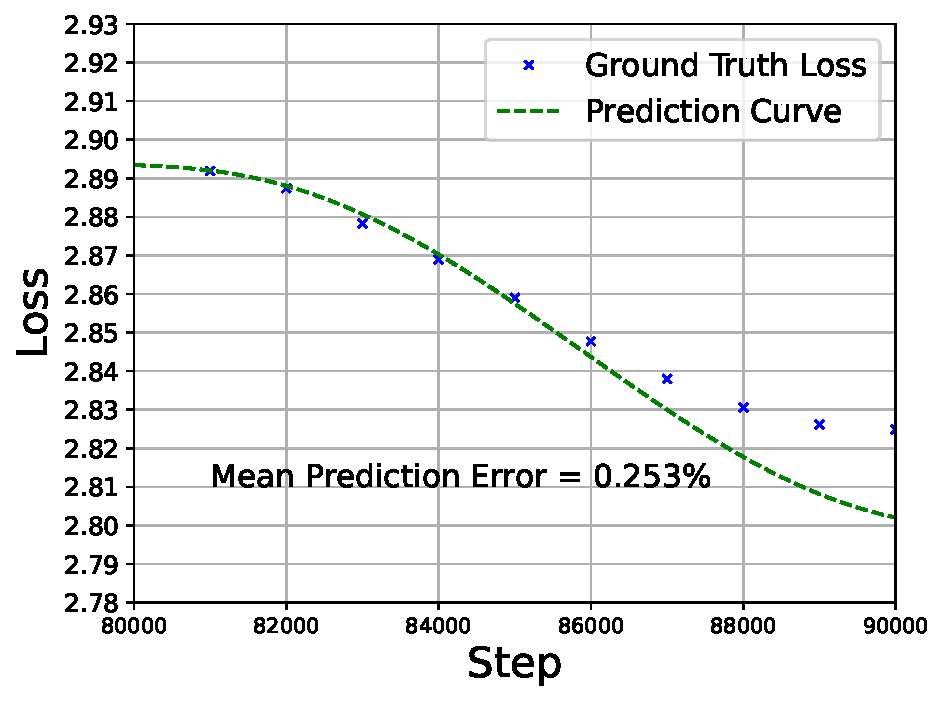
\includegraphics[width=0.32\textwidth]{images/plot_newxy/12w_predict_WSDW-80000-cosine-90000-cosine-100000_zoomin.pdf}
        \caption{Full curve prediction of WSD LRS (90K total steps; 10 \% cosine annealing to $\eta_{min} = 0$).}
        \label{fig:prediction-9w-wsd}
    \end{subfigure}

    \begin{subfigure}[b]{\textwidth}
        \centering
        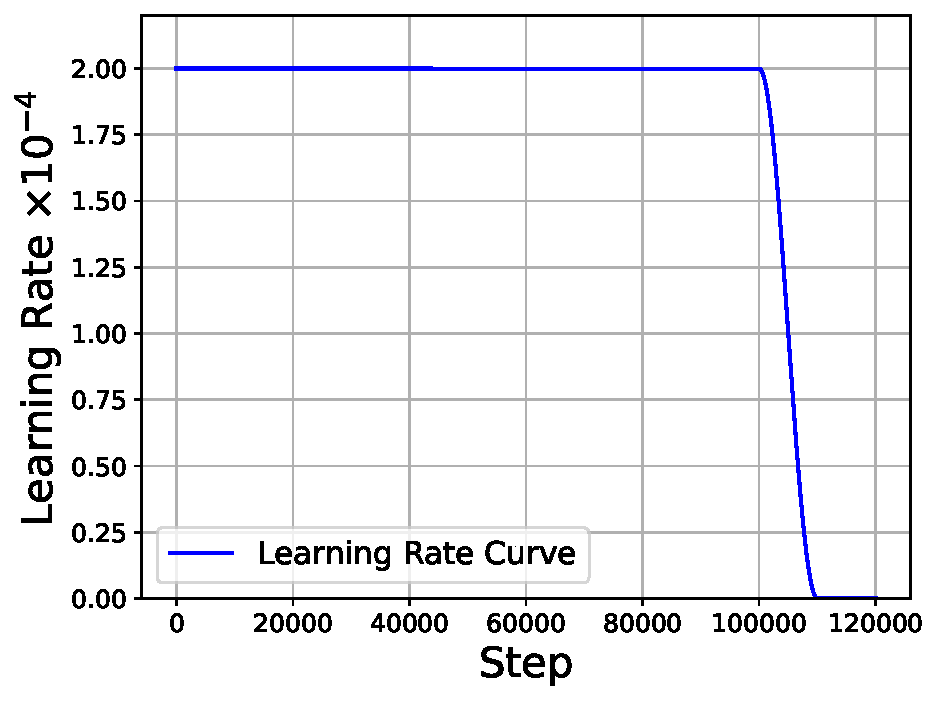
\includegraphics[width=0.32\textwidth]{images/plot_newxy/12w_lr_wsd_1.pdf}
        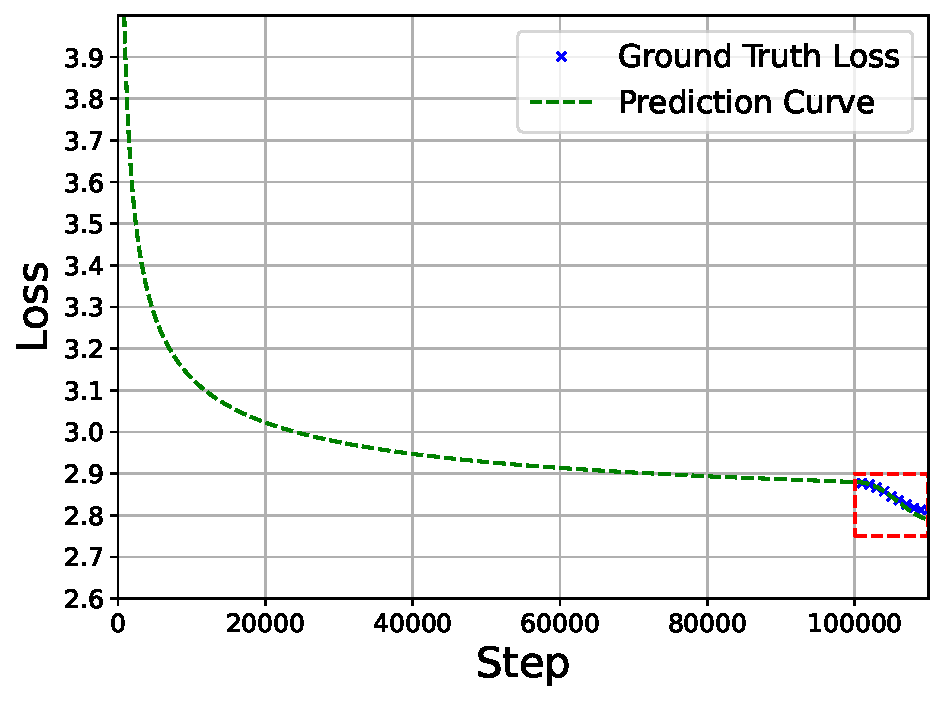
\includegraphics[width=0.32\textwidth]{images/plot_newxy/12w_predict_WSDW-100000-cosine-110000-cosine-120000_zoomout.pdf}
        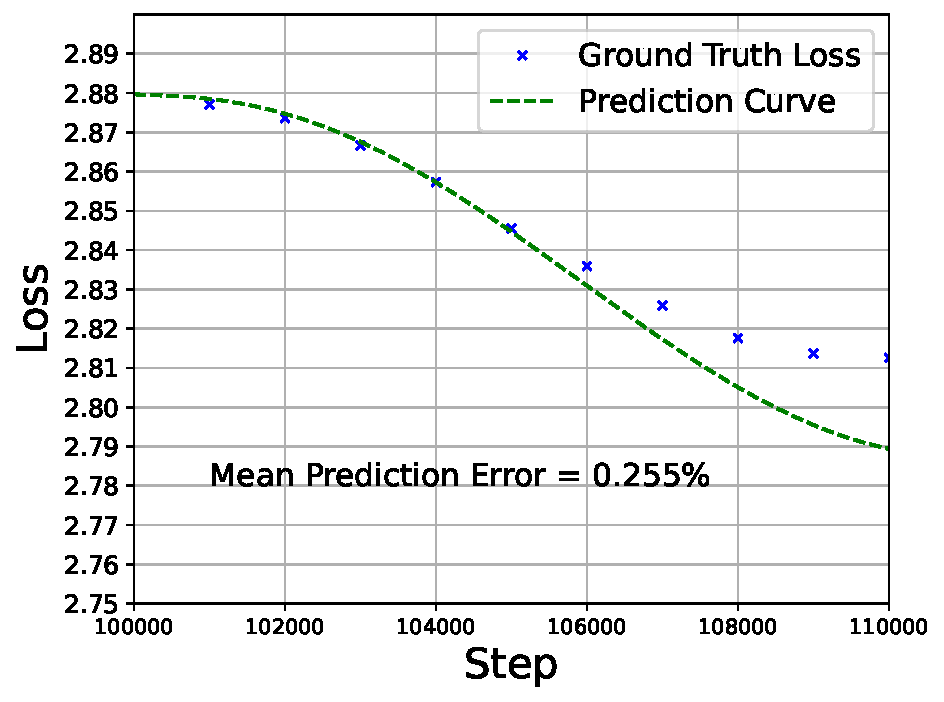
\includegraphics[width=0.32\textwidth]{images/plot_newxy/12w_predict_WSDW-100000-cosine-110000-cosine-120000_zoomin.pdf}
        \caption{Full curve prediction of WSD LRS (110K total steps; 10 \% cosine annealing to $\eta_{min} = 0$).}
        \label{fig:prediction-11w-wsd}
    \end{subfigure}
    
    \caption{Using the fitted equation in Fig.~\ref{fig:fit_12w} to \textbf{predict} full loss curves for unseen LRS with 120K total steps. The left, medium, and right columns represent LR curve, the predicted loss curves, and a zoomed-in view of loss curve, respectively. The red rectangle indicates the zoomed-in zone. Warmup steps (100) are not shown in this figures. 
    Notable, all LRS and loss curves shown here were \textbf{unseen} during the fitting process. The mean prediction errors across different LRS is as low as $\sim 0.2\%$. Refer to setting B in Table~\ref{tab:exp-sets} for detailed experimental setups.}
\label{fig:predict_12w}
\end{figure}

\subsection{Experiments on the Mixture of Experts Architecture}
\label{apx:moe}
% Fig.~\ref{fig:fit} and Fig.~\ref{fig:prediction} show that our equation can work very well on the dense Llama-like architecture~\citep{vaswani2017attention,touvron2023llama}.
We validate our equation on the Mixture of Experts (MoE) architecture.
The experimental setting is shown as setting $D$ in Table~\ref{tab:exp-sets}.
We add the widely-used auxiliary loss for load balancing among experts~\citep{fedus2021switch}. Moreover, we change the LRS and total steps to 60K WSD with 10K annealing steps in fitting, testing whether our scaling law is effective
under various circumstances.
The fitting results shown in Fig.~\ref{fig:moe_fit} and the prediction results shown in Fig.~\ref{fig:moe_prediction} indicates that our equation still works well on the MoE architecture.

\begin{figure}[p]
    \centering
    \begin{subfigure}[b]{0.32\textwidth}
        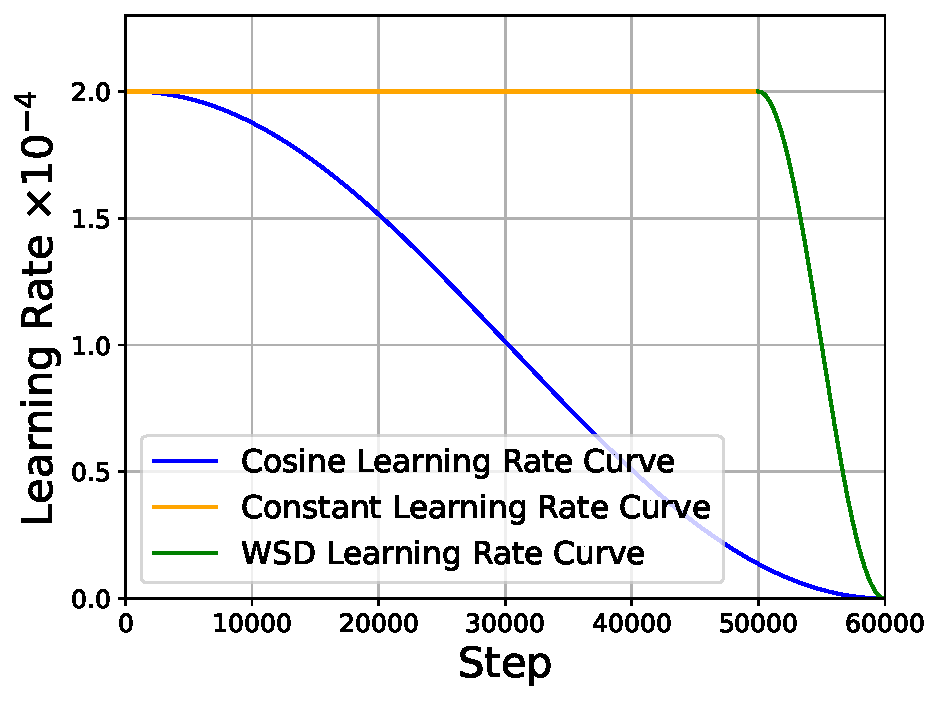
\includegraphics[width=\textwidth]{images/plot_newxy/lr_moe.pdf}
        \caption{Learning rate.}
    \end{subfigure}
    \hfill
    \begin{subfigure}[b]{0.32\textwidth}
        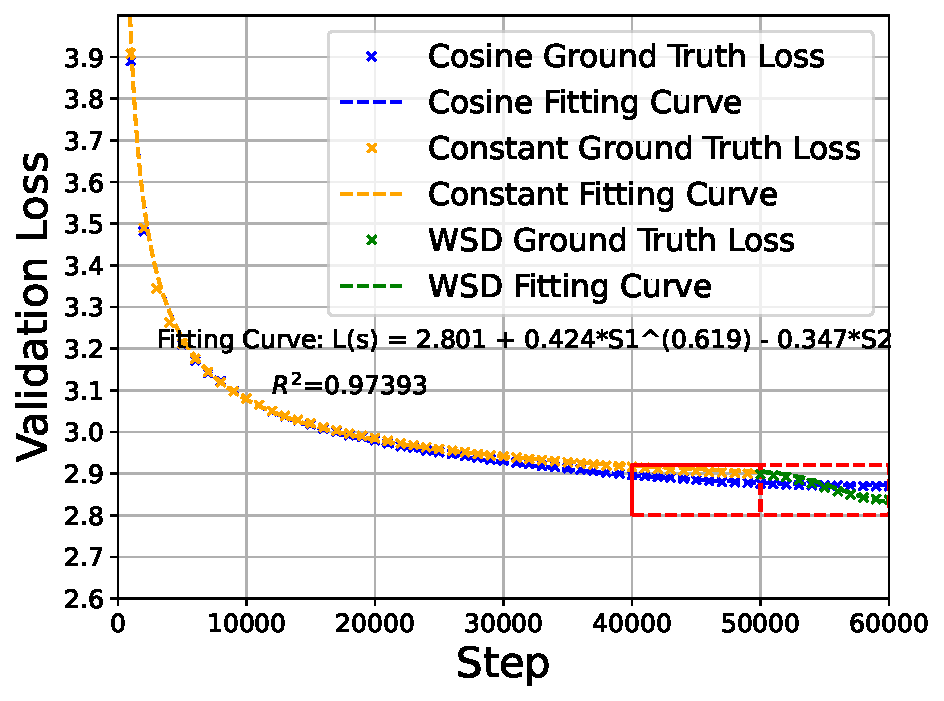
\includegraphics[width=\textwidth]{images/plot_newxy/all_predict_WSD-50000-cosine-60000_zoomout.pdf}
        \caption{Zoomed-out loss fitting.}
    \end{subfigure}
    \hfill
    \begin{subfigure}[b]{0.32\textwidth}
        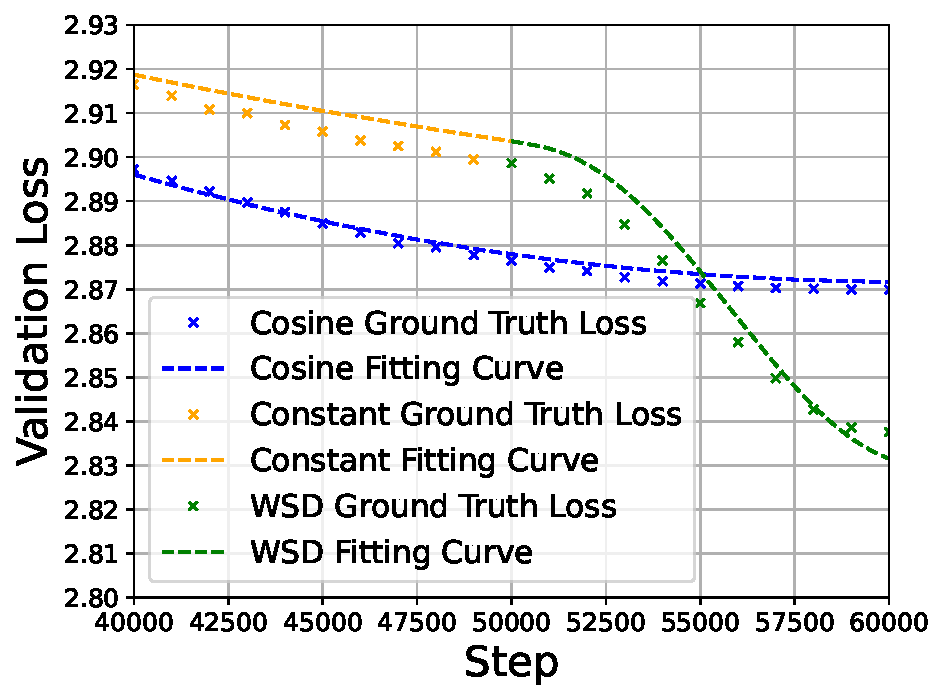
\includegraphics[width=\textwidth]{images/plot_newxy/all_predict_WSD-50000-cosine-60000_zoomin.pdf}
        \caption{Zoomed-in loss fitting.}
    \end{subfigure}
    \caption{Full loss curve \textbf{fitting} for MoE models. After fitting, we get a \textbf{universal} loss equation $L = 2.801 + 0.424\cdot S_1^{-0.619} - 0.347\cdot S_2$. Refer to setting D in Table~\ref{tab:exp-sets} for detailed experimental setups.}
\label{fig:moe_fit}
\end{figure}


\begin{figure}[tbp]
    \centering
    
    \begin{subfigure}[b]{\textwidth}
        \centering
        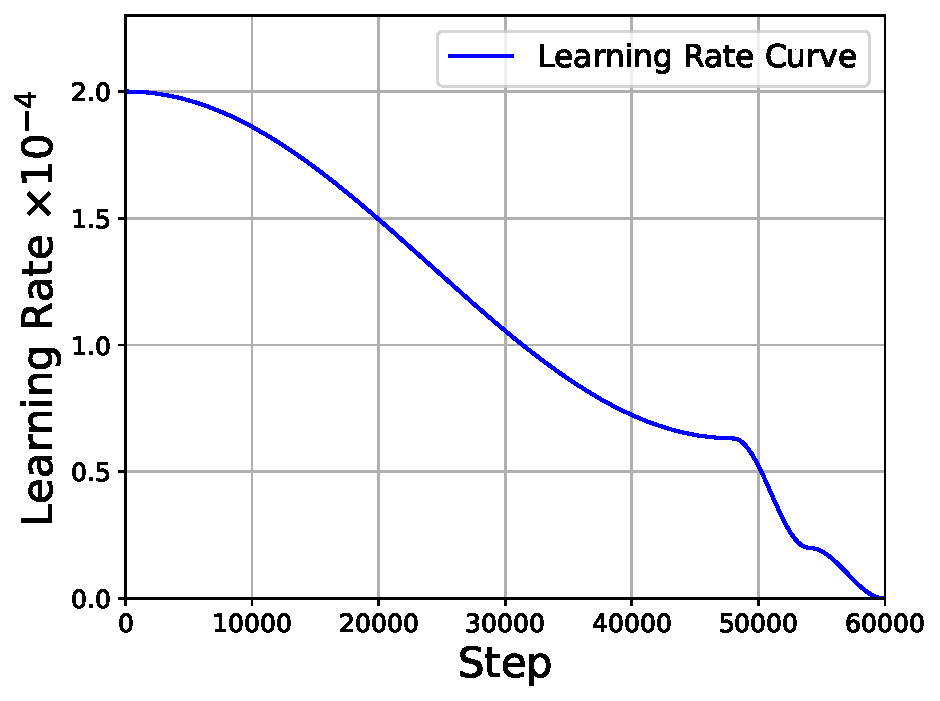
\includegraphics[width=0.32\textwidth]{images/plot_newxy/lr_moe_split.pdf}
        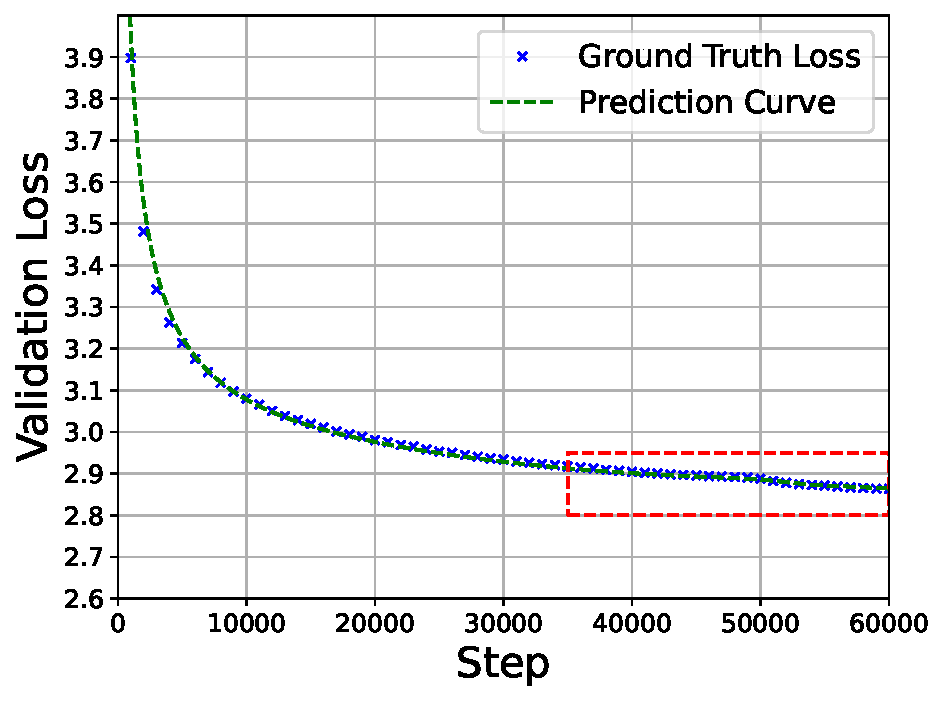
\includegraphics[width=0.32\textwidth]{images/plot_newxy/bll_predict_split-500-48000-0.316-54000-0.1-60000-0.0_zoomout.pdf}
        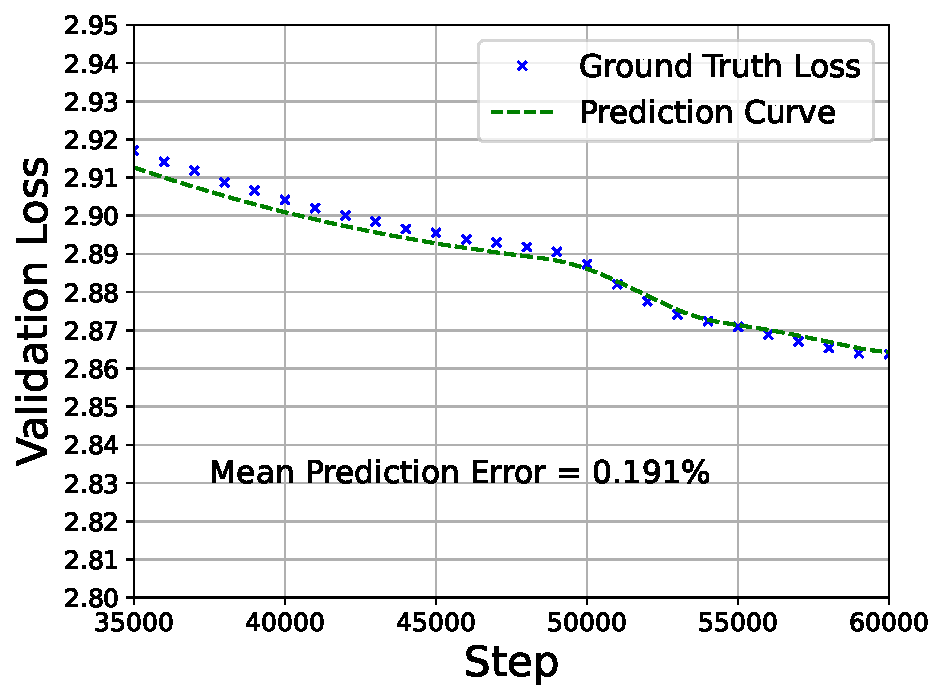
\includegraphics[width=0.32\textwidth]{images/plot_newxy/bll_predict_split-500-48000-0.316-54000-0.1-60000-0.0_zoomin.pdf}
        \caption{Full curve prediction of multi-step cosine LRS (80\% + 10\% + 10\%)~\citep{deepseek-ai2024deepseek}}
        \label{fig:moe_prediction-multi-cosine}
    \end{subfigure}

    \begin{subfigure}[b]{\textwidth}
        \centering
        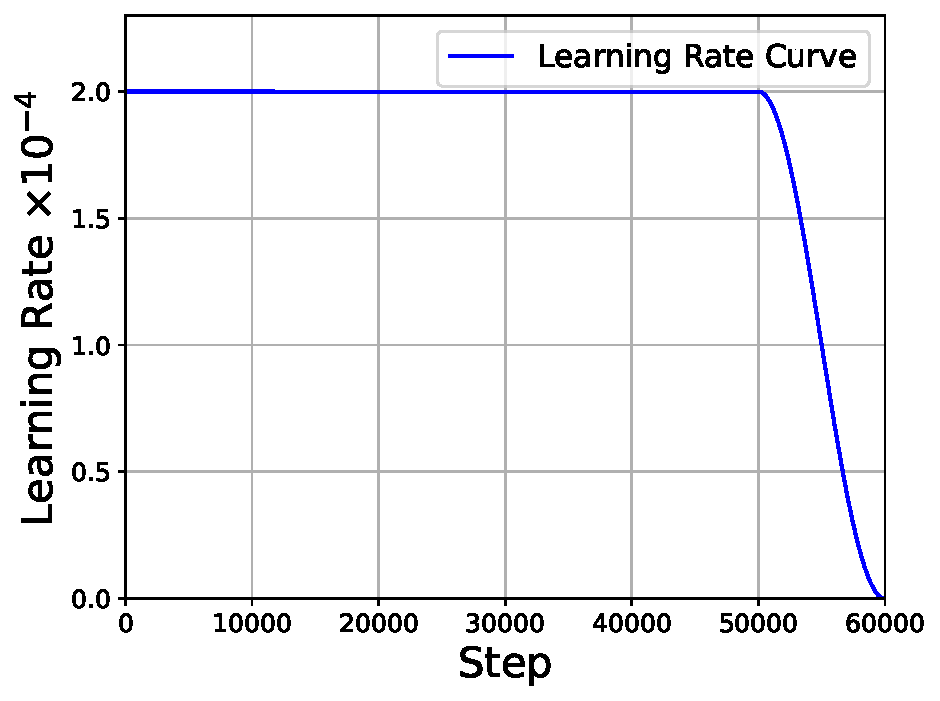
\includegraphics[width=0.32\textwidth]{images/plot_newxy/lr_moe_wsd.pdf}
        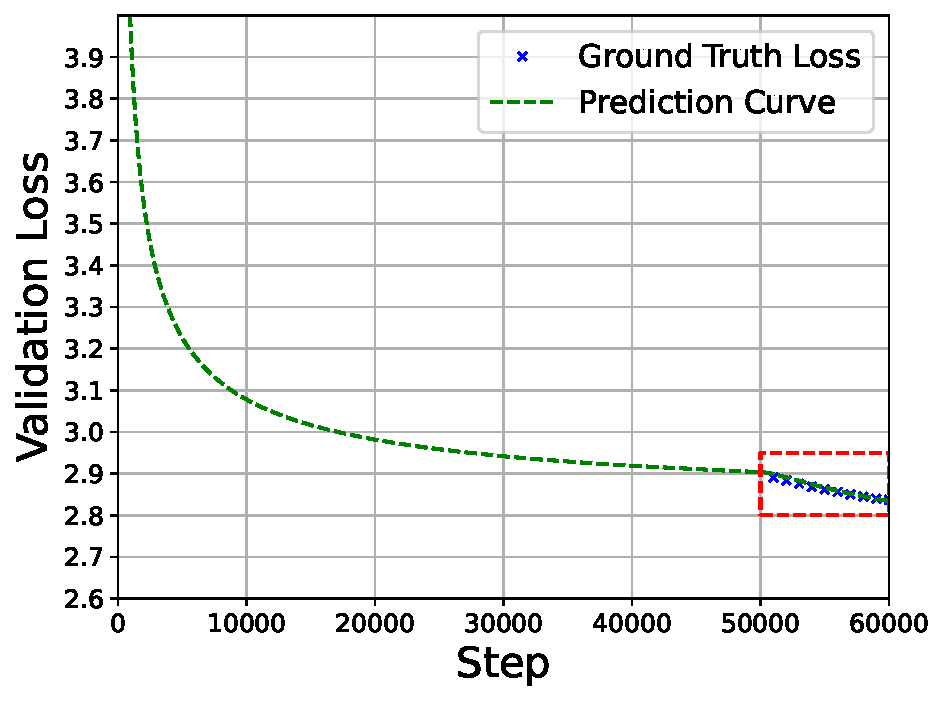
\includegraphics[width=0.32\textwidth]{images/plot_newxy/bll_predict_WSD-50000-exponential-60000_zoomout.pdf}
        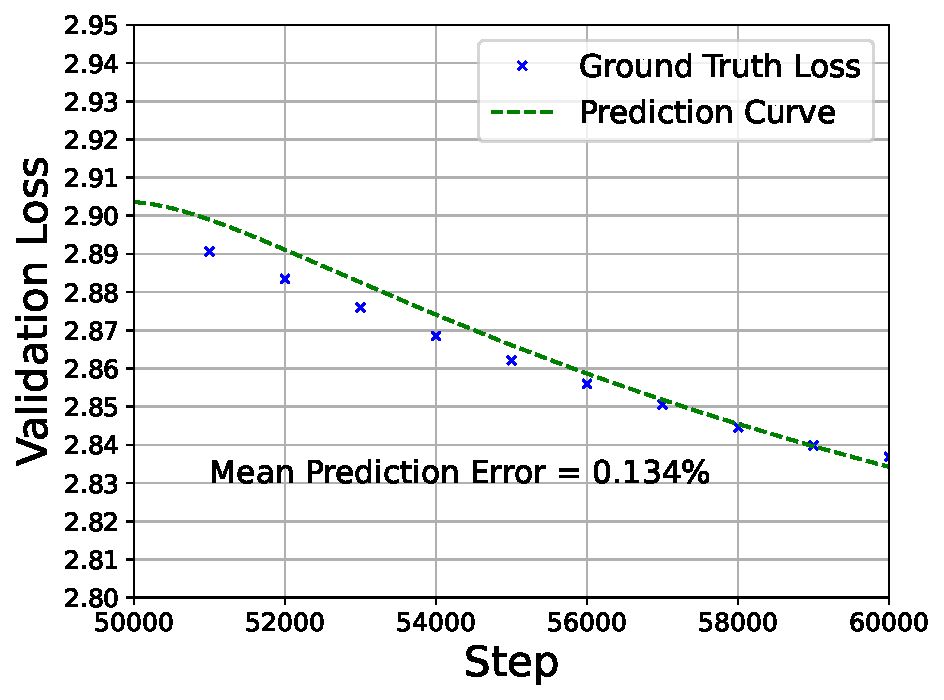
\includegraphics[width=0.32\textwidth]{images/plot_newxy/bll_predict_WSD-50000-exponential-60000_zoomin.pdf}
        \caption{Full curve prediction of WSD LRS (17\% exponential annealing to $\eta_{min} = 0$)~\citep{hu2024minicpm}.}
        \label{fig:moe_prediction-wsd}
    \end{subfigure}
    
     \begin{subfigure}[b]{\textwidth}
        \centering
        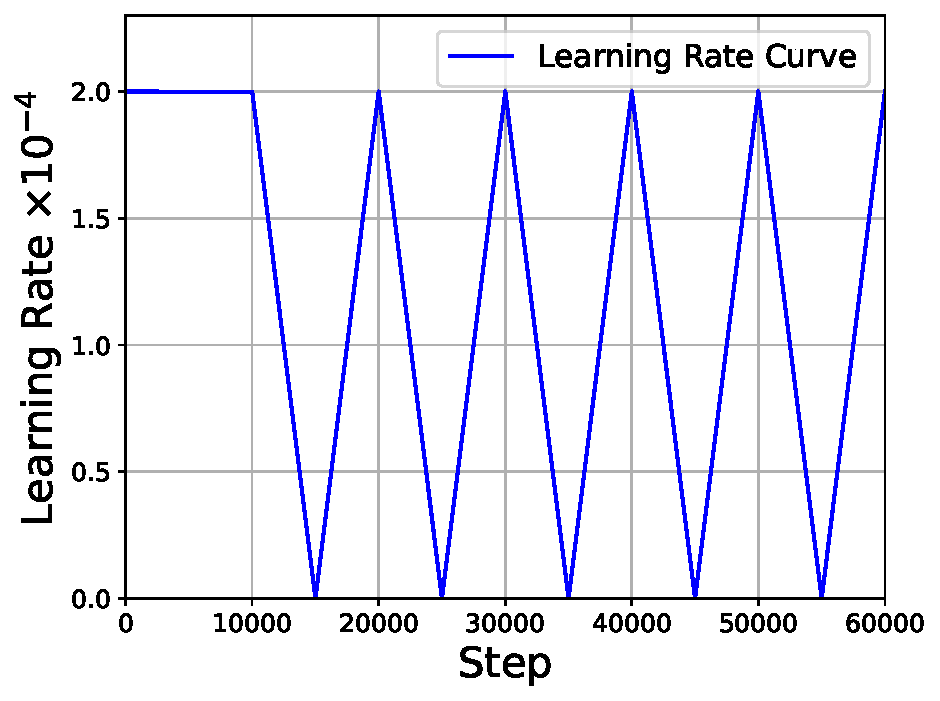
\includegraphics[width=0.32\textwidth]{images/plot_newxy/lr_moe_linear.pdf}
        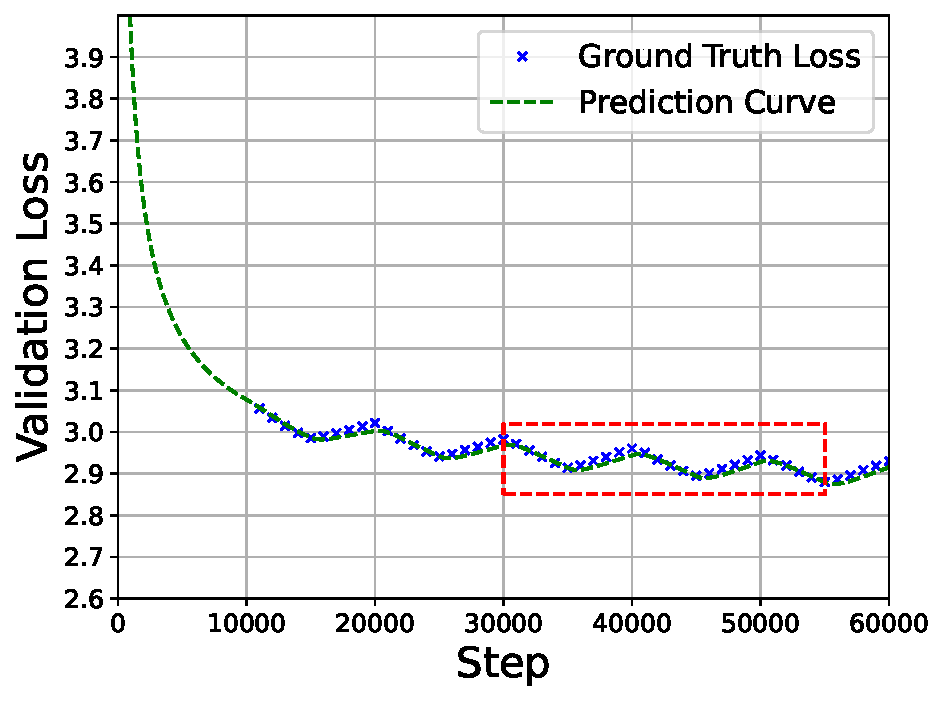
\includegraphics[width=0.32\textwidth]{images/plot_newxy/bll_predict_all-10000-linear-5000-linear-5000_zoomout.pdf}
        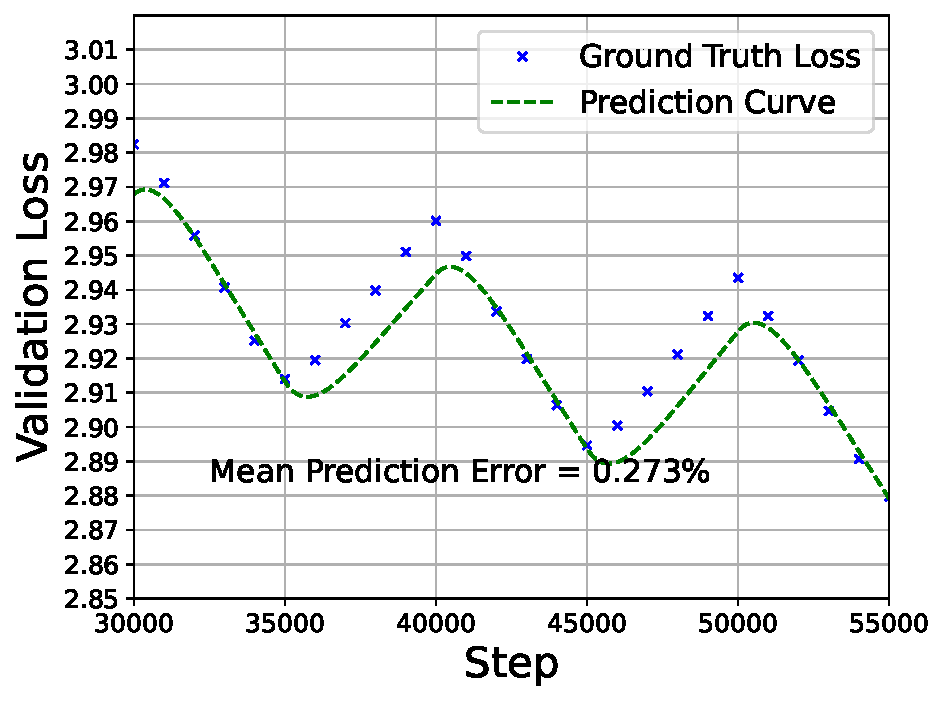
\includegraphics[width=0.32\textwidth]{images/plot_newxy/bll_predict_all-10000-linear-5000-linear-5000_zoomin.pdf}
        \caption{Full curve prediction of Cyclic LRS~\citep{smith2017cyclical} including multiple unseen LR re-warmup stages.}
        \label{fig:moe_prediction-strange}
    \end{subfigure}
    
    \caption{Using the fitted equation in Fig.~\ref{fig:moe_fit} to \textbf{predict} full loss curves for unseen LRS (MoE model). The left, medium, and right columns represent LR curve, the predicted loss curves and a zoomed-in view of loss curves, respectively. 
    The red rectangle indicates the zoomed-in zone. Warmup steps (500) are not shown in this figure. 
    Noteable, all LRS and loss curves shown here were unseen during the fitting process. The mean prediction errors across different LRS is as low as $\sim 0.2\%$. Refer to setting D in Table~\ref{tab:exp-sets} for detailed experimental setups.
    }
\label{fig:moe_prediction}
\end{figure}

\subsection{Scaling Up for Much Longer Steps}
\label{apx:long-exp}
In this section, we validate the effectiveness of our equation in predicting loss curves over significantly long total steps. This scalability is particularly useful in large-scale training.
Specifically, we fit our equation on loss curves yield by the constant and cosine LRS with 30K steps and predict the loss curve for the WSD LRS with 350K steps. The model has 1.7 billion parameters, and the training uses 1,400 billion tokens. More detailed experimental setup is shown as the setting $E$ in Table~\ref{tab:exp-sets}. 

The fitting and prediction results are shown in Fig.~\ref{fig:35_fit} and Fig.~\ref{fig:35_predict} respectively. It shows that we accurately predict the loss curve for the annealing stage after 10x longer steps in advance.


\begin{figure}[p]
    \centering
    \begin{subfigure}[b]{0.32\textwidth}
        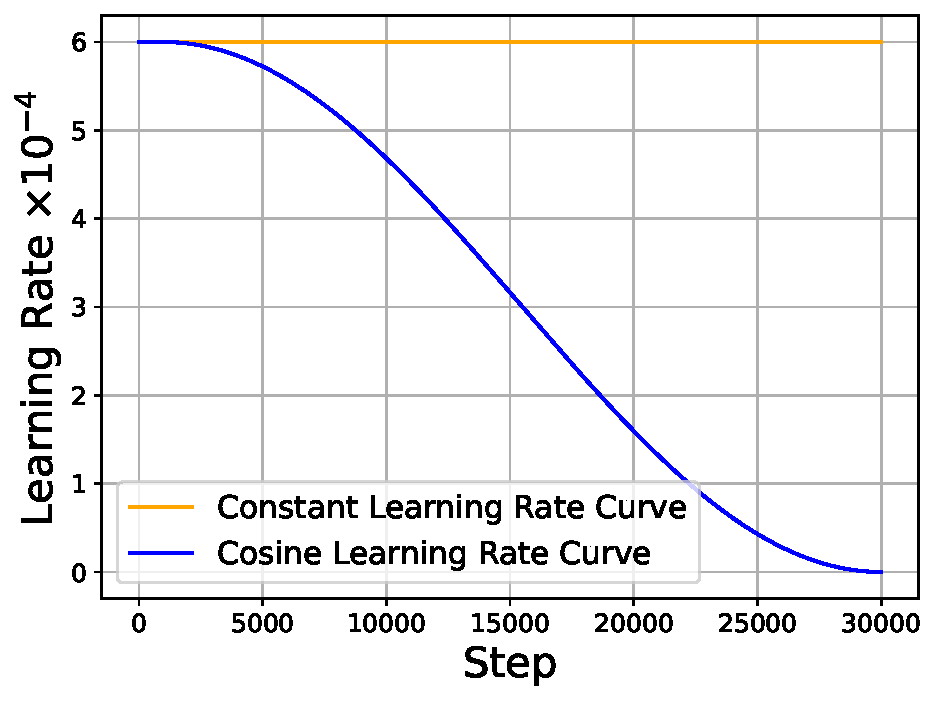
\includegraphics[width=\textwidth]{images/plot_newxy/lr_35_all.pdf}
        \caption{Learning rate.}
    \end{subfigure}
    \hfill
    \begin{subfigure}[b]{0.32\textwidth}
        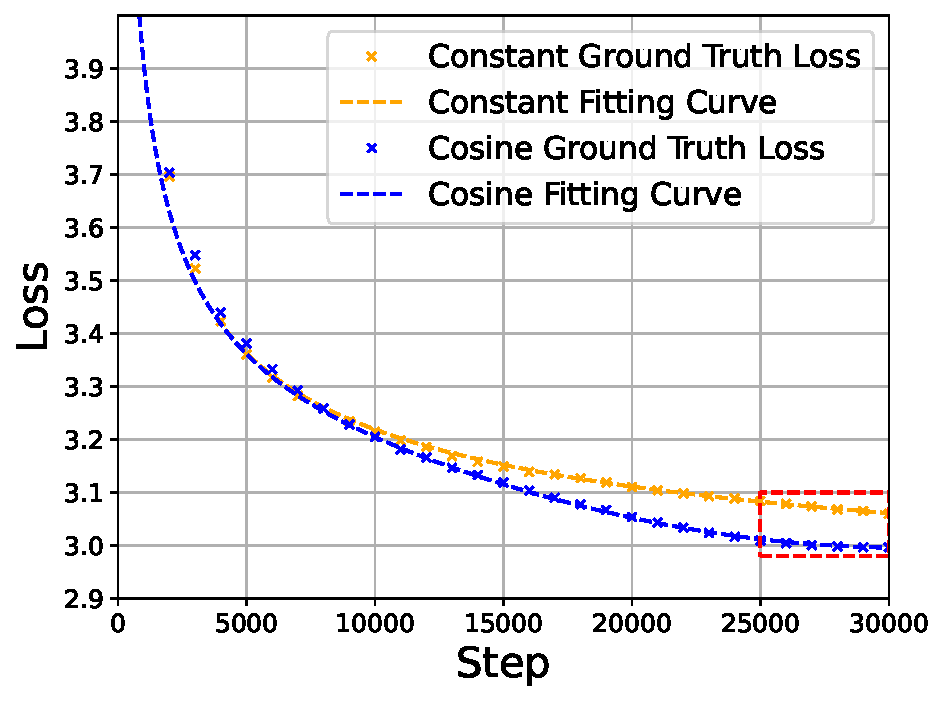
\includegraphics[width=\textwidth]{images/plot_newxy/35_fit_zoomout.pdf}
        \caption{Zoomed-out loss fitting.}
    \end{subfigure}
    \hfill
    \begin{subfigure}[b]{0.32\textwidth}
        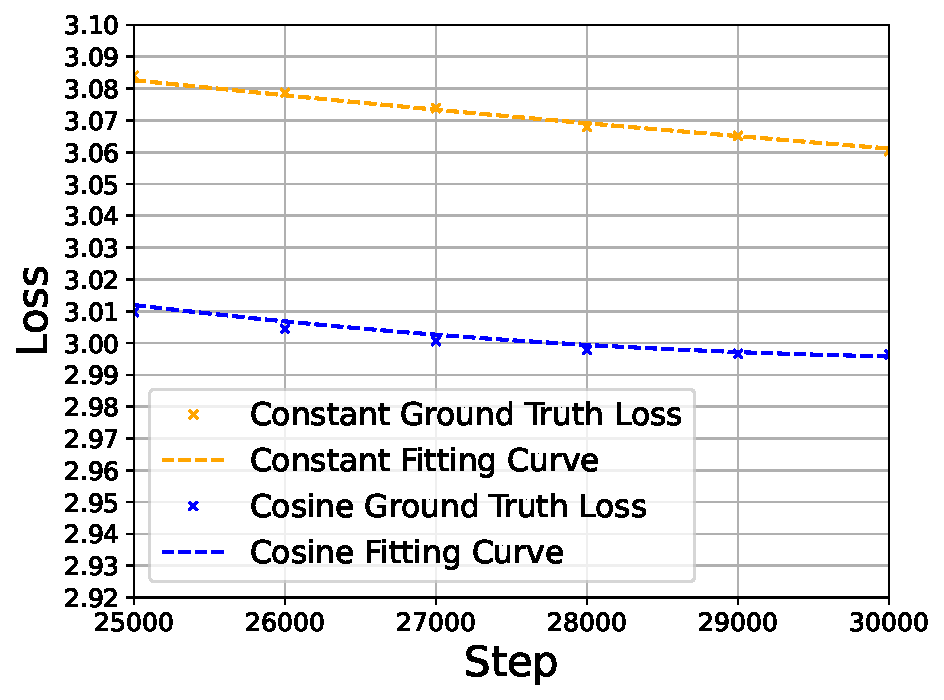
\includegraphics[width=\textwidth]{images/plot_newxy/35_fit_zoomin.pdf}
        \caption{Zoomed-in loss fitting.}
    \end{subfigure}
    \caption{Full loss curve \textbf{fitting} for the constant and cosin LRS on 30K steps. After fitting, we get a \textbf{universal} loss equation $L = 2.788 + 0.906\cdot S_1^{-0.416} - 0.254\cdot S_2$. Refer to setting E in Table~\ref{tab:exp-sets} for detailed experimental setups. }
\label{fig:35_fit}
\end{figure}


\begin{figure}[tbp]
    \centering
    \begin{subfigure}[b]{0.32\textwidth}
        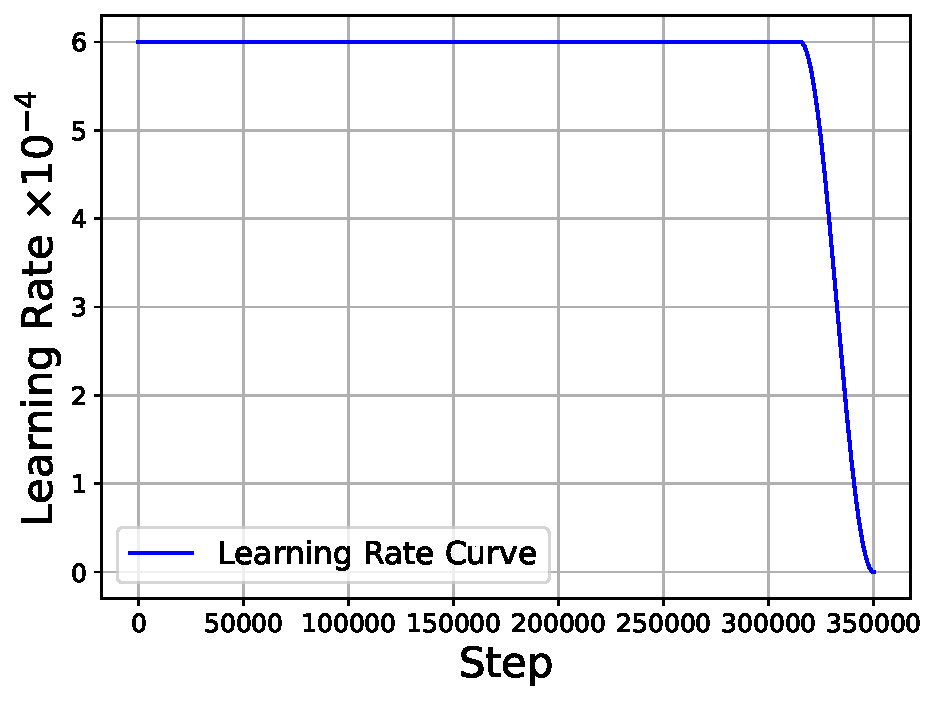
\includegraphics[width=\textwidth]{images/plot_newxy/lr_35_wsd.pdf}
        \caption{Learning rate.}
    \end{subfigure}
    \hfill
    \begin{subfigure}[b]{0.32\textwidth}
        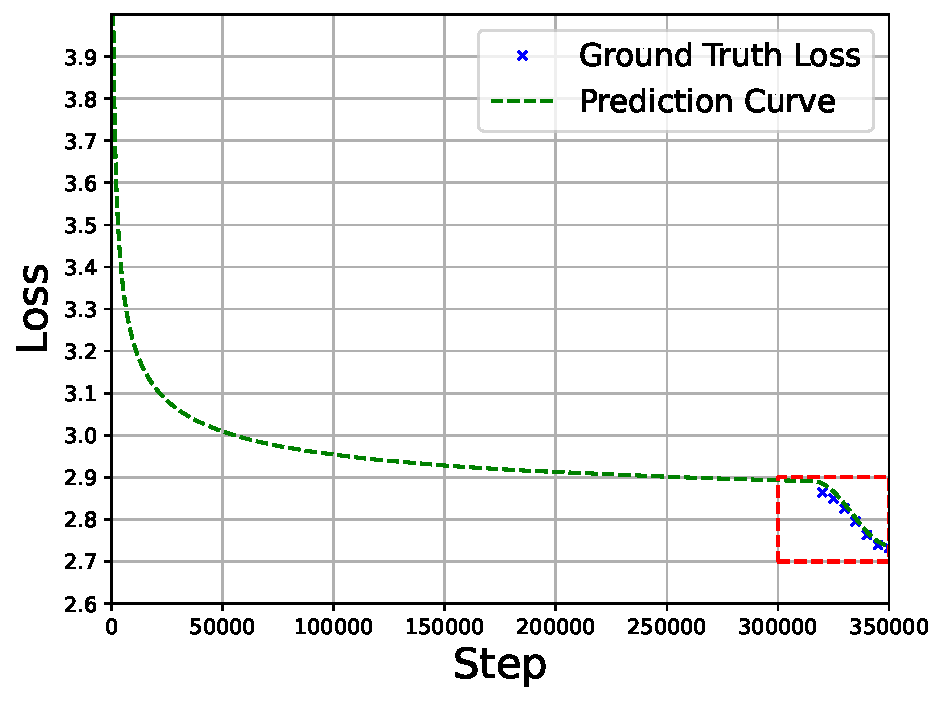
\includegraphics[width=\textwidth]{images/plot_newxy/predict_WSD-315000-cosine-350000_zoomout.pdf}
        \caption{Zoomed-out loss prediction.}
    \end{subfigure}
    \hfill
    \begin{subfigure}[b]{0.32\textwidth}
        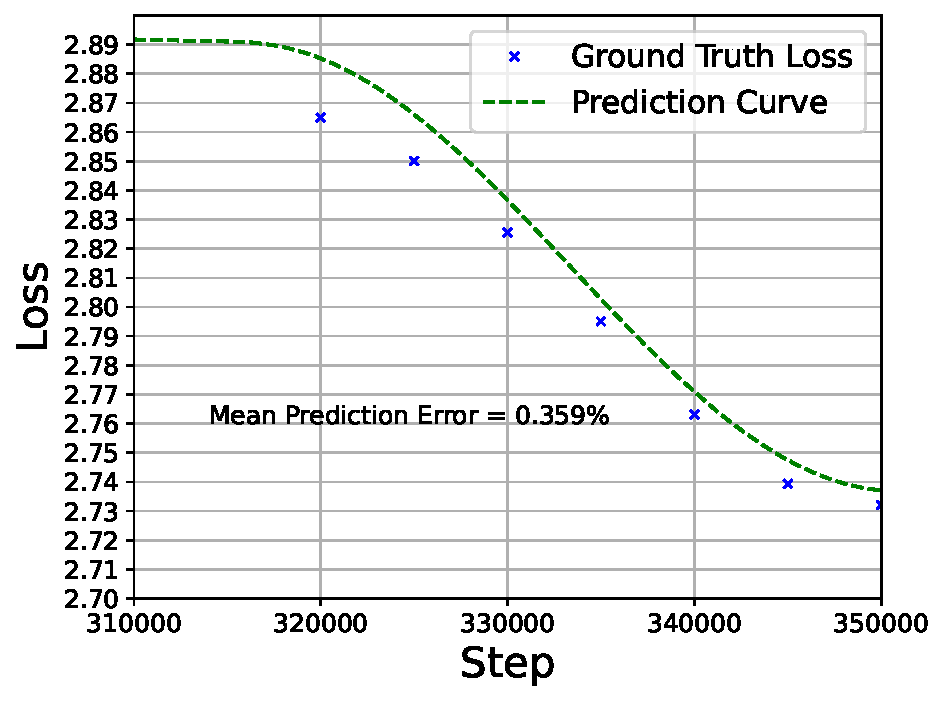
\includegraphics[width=\textwidth]{images/plot_newxy/predict_WSD-315000-cosine-350000_zoomin.pdf}
        \caption{Zoomed-in loss prediction.}
    \end{subfigure}
    \caption{Using the fitted equation in Fig.~\ref{fig:35_fit} to \textbf{predict} the full loss curve equation under the WSD LRS (10\% cosine annealing ratio to $\eta_{min}=0$). Our equation accurately predict the loss curve in the annealing stage after the 10x longer steps. Refer to setting E in Table~\ref{tab:exp-sets} for detailed experimental setups.}
\label{fig:35_predict}
\end{figure}

\subsection{Open-sourced Models}
\label{apx:open-source}
To further validate our proposed scaling law, we apply our equation on modeling the loss curves of open-sourced language models, including BLOOM-176B~\citep{workshop2022bloom} and OLMo-1B~\citep{groeneveld2024olmo}. As shown in Fig.~\ref{fig:open-source-fit}, our equation fits very well on loss curves of open-sourced models, even when the model size scales up to 176B (e.g. BLOOM) and token number scales up to 2000B over 740K steps (e.g. OLMo). 

\begin{figure}[tbp]
    \centering
    \begin{subfigure}[b]{0.48\textwidth}
        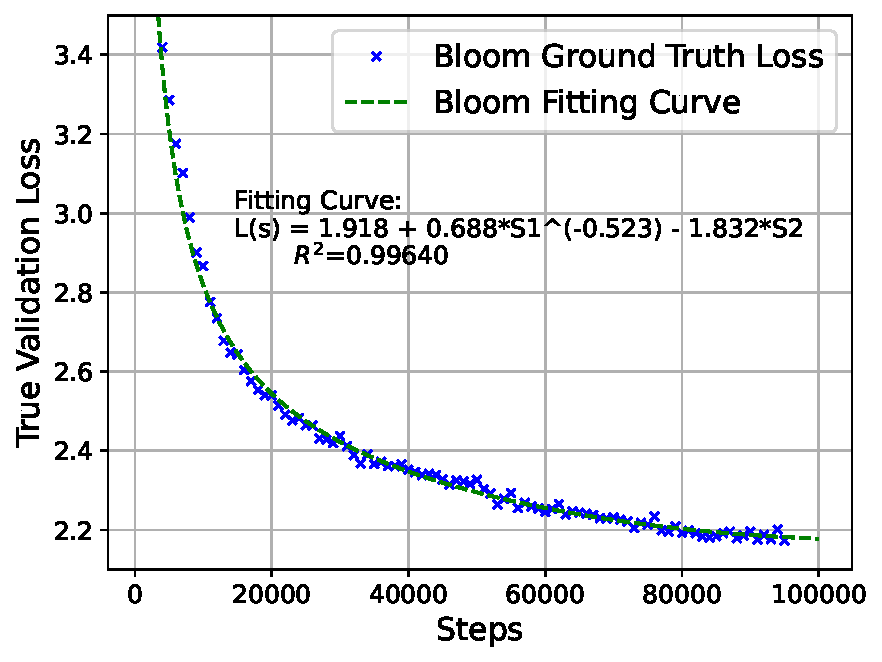
\includegraphics[width=\textwidth]{images/plot_new/bloom.pdf}
        \caption{Full loss curve fitting on BLOOM-176B.}
        \label{fig:bloom}
    \end{subfigure}
    \hfill
    \begin{subfigure}[b]{0.48\textwidth}
        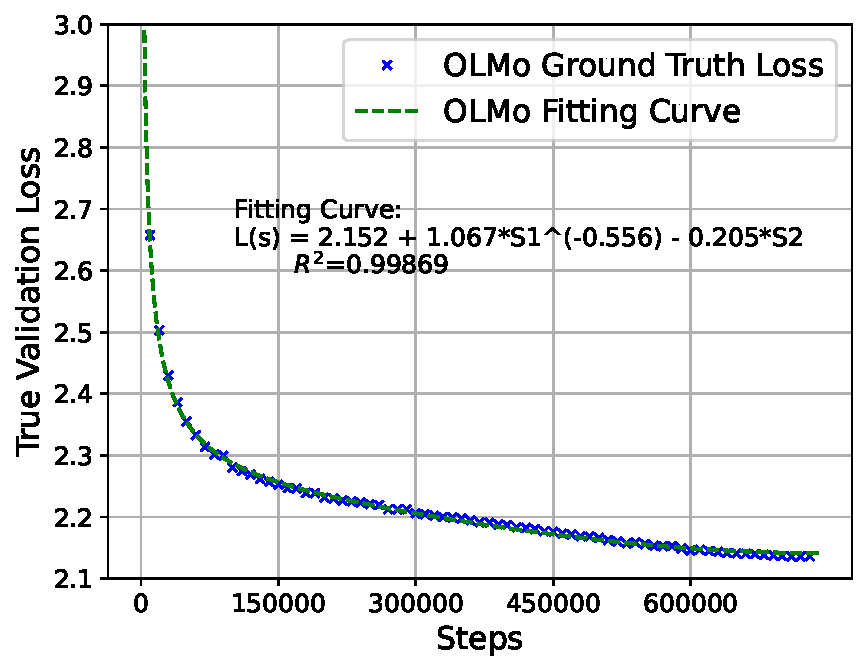
\includegraphics[width=\textwidth]{images/plot_new/olmo.pdf}
        \caption{Full loss curve fitting on OLMo-1B (2T tokens).}
        \label{fig:olmo}
    \end{subfigure}
    \caption{Fitting loss curves for open sourced models. We extract the curve of BLOOM from \url{https://huggingface.co/bigscience/bloom/tensorboard}, and choose the column \texttt{lm-loss-validation/valid/lm loss validation} as the validation loss.
    We extract the curve of OLMo from {\url{https://wandb.ai/ai2-llm/OLMo-1B?nw=nwuserdirkgr}, and choose the column \texttt{eval/pile/CrossEntropyLoss} as the validation loss.
    Both models adopt cosine LRS.}
    }
\label{fig:open-source-fit}
\end{figure}



\subsection{Our $N$-extended Scaling Law on Another Experiments Setups}
\label{apx:exp-2-N}
Fig.~\ref{fig:scaling-N-fit} shows that our $N$-extended equation (Eq.~\ref{eq:scaling-N}) works well on our main experimental setup.
Similarly, to validate the effectiveness of our $N$-extended scaling equation on various different experimental settings, we change our setup from setting $A$ to setting $C$ (refer to Table~\ref{tab:exp-sets}). The fitting results are shown in Fig.~\ref{fig:extend-N-apx}. The results suggest that our $N$-extended scaling law with LR annealing works well across different experimental setups.

\begin{figure}[tbp]
\centering
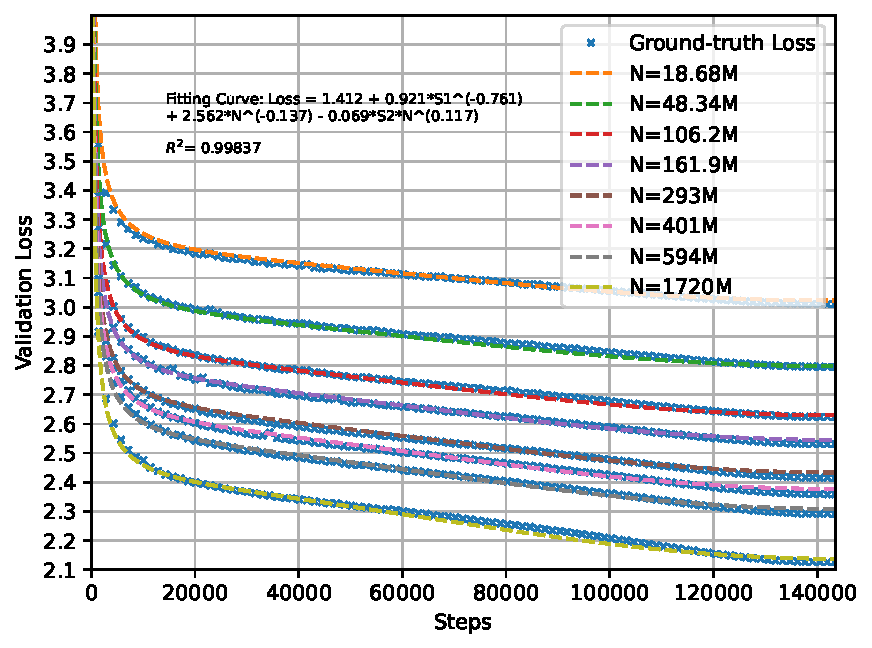
\includegraphics[width=0.7\textwidth]{images/draw_phe/6-2.pdf}
\caption{Curve fitting on cosine LRS (143K steps to $\eta_{min}=0$) for various different model sizes using our scaling law extended to model size $N$. Refer to setting C in Table~\ref{tab:exp-sets} for detailed experimental setups.}
\label{fig:extend-N-apx}
\end{figure}

% \section{Comparison with Chinchilla Scaling Law}
% \subsection{Reduction to Chinchilla Scaling Law}
% \label{apx:reduction}
% We have proved that our scaling law can be reduced to chinchilla scaling law for constant LRS in Sec.~\ref{sec:comparison}.
% For other LRS, we adopt a method based on statistics to show that our scaling law function can be reduced to the chinchilla scaling law. 
% Specifically, we check whether the chinchilla scaling law equation can fit the endpoints of loss curves predicted by our scaling law.
% The parameter tuple of our equation is $(L_{0}, A, C, \alpha)$. We then randomly sample 1000 sets of parameter tuples from some uniform distributions:
% $L_0\sim U(1,3)$, $A\sim U(0.3,0.5)$, $C\sim U(0.2,0.6)$,  $\alpha\sim U(-0.6,-0.4)$.
% Each parameter tuple could be seen as the fitting result of a distinct set of experimental setups~\footnote{It's worth noting that some of these sampled parameter tuples might not be reasonable or un-likely to be observed in real experiments, but we choose to keep them nonetheless.}. (e.g. dataset, batch size, model size, etc.).
% For each generated parameter tuple, we apply our equation to predict the final loss of different total training steps on two LRS including cosine and WSD (10\% annealing ratio), 
% ranging from 5K to 60K steps. 
% The predicted loss values on final steps are used to fit the chinchilla equation. 
% The fitting results are shown in Fig.~\ref{fig:phe-reduction}.

% \begin{figure}[tbp]
%     \centering
%     \begin{subfigure}[b]{0.48\textwidth}
%         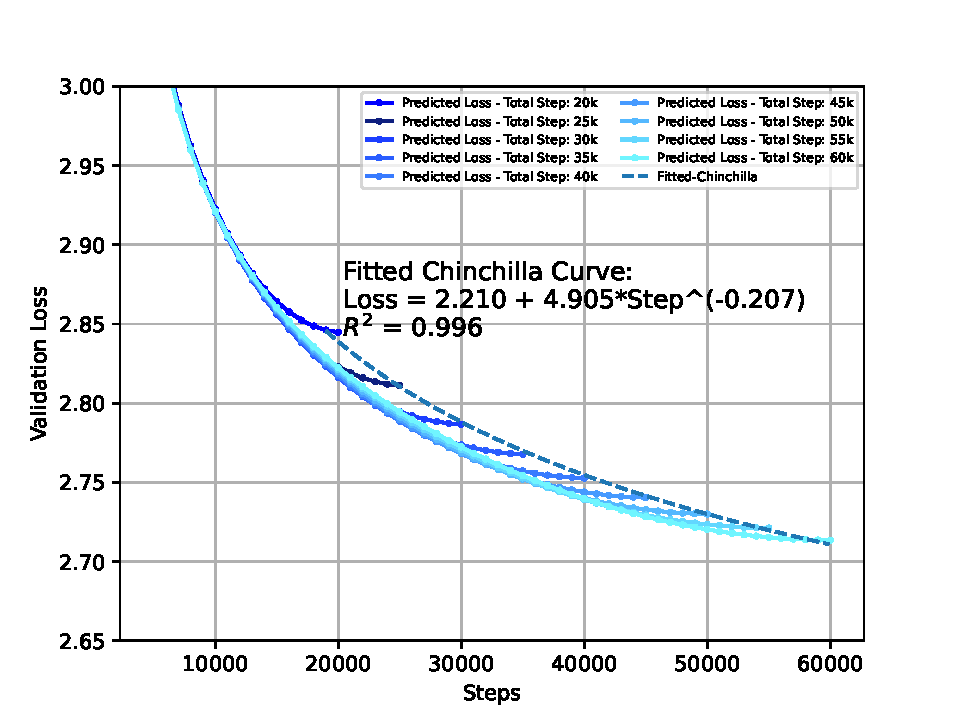
\includegraphics[width=\textwidth]{images/reduce_cosine.pdf}
%         \caption{The predicted loss of different total steps with cosine LRS and the fitted chinchilla curve.}
%     \end{subfigure}
%     \hfill
%     \begin{subfigure}[b]{0.48\textwidth}
%         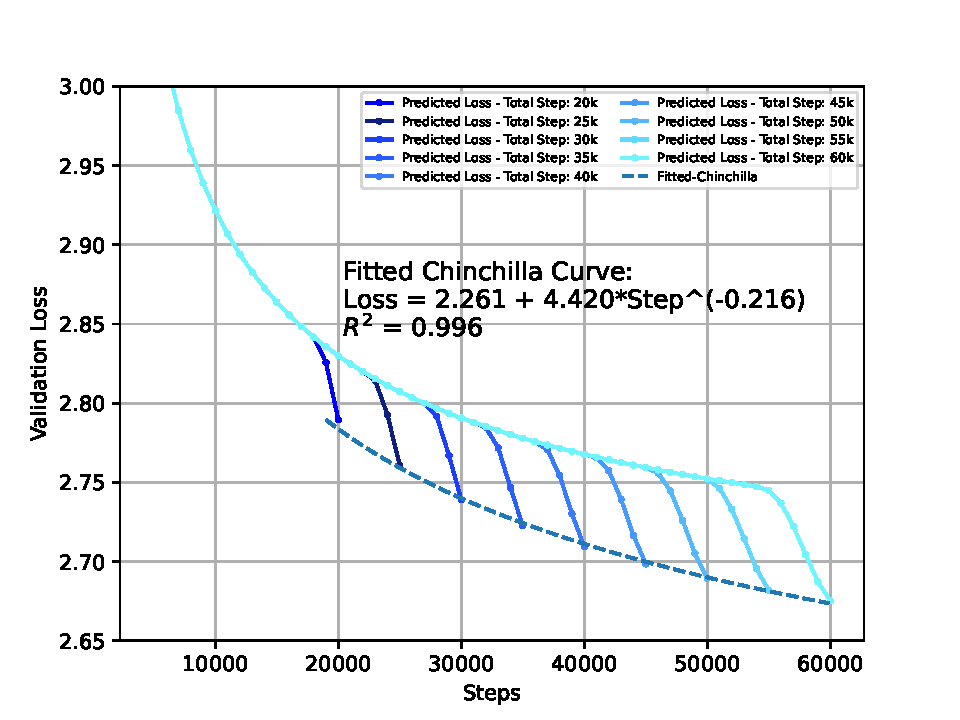
\includegraphics[width=\textwidth]{images/reduce_wsd.pdf}
%         \caption{The predicted loss of different total steps with WSD LRS and the fitted chinchilla curve.}
%     \end{subfigure}
%     \caption{The Chinchilla scaling law equation fits well on the final validation losses predicted by our formulation, taking cosine LRS (on the left) and WSD LRS (on the right) as examples.}
% \label{fig:phe-reduction}
% \end{figure}

% \subsection{Scaling Law Computational Cost Comparison}
% \label{apx:green}
% We compare the computational cost required by different scaling law formulations in this section.
% Specifically, we evaluate the computational cost of obtaining 100 fitting points for each scaling law equation with an step interval of $K$, i.e. the total parameter updates performed to obtain the validation loss at the $1K, 2K, \dots, 100K$ steps: 
% \begin{itemize}
%     \item Fitting the \textbf{Chinchilla scaling law equation with the cosine LRS} requires a total number of parameter updates of $1K + 2K + 3K + \cdots + 100K = 5050K$;
%     \item Fitting the \textbf{Chinchilla scaling law equation with the WSD LRS} requires a total number of parameter updates of $(1K + 2K + 3K + \cdots + 100K)r + 100K(1-r) = (100 + 4950r)K$, in which $r$ is the annealing ratio for the WSD LRS.
%     \item Fitting \textbf{our scaling law equation} only need one training curve with a moderate number of parameter updates, such as one curve under the cosin LRS with $50K$ training steps. Further, the number of loss values we can get for fitting our equation are far more than $100$. Note that more fitting points generally achieve more accurate fitting results. Our equation can also utilize loss curves from various different LRS.
% \end{itemize}

% It can be seem that our formulation requires far less computations comparing to other approaches.

\section{WSD Scheduler and Annealing Functions}

\begin{figure}[tbp]
    \centering
    \begin{subfigure}[b]{0.48\textwidth}
        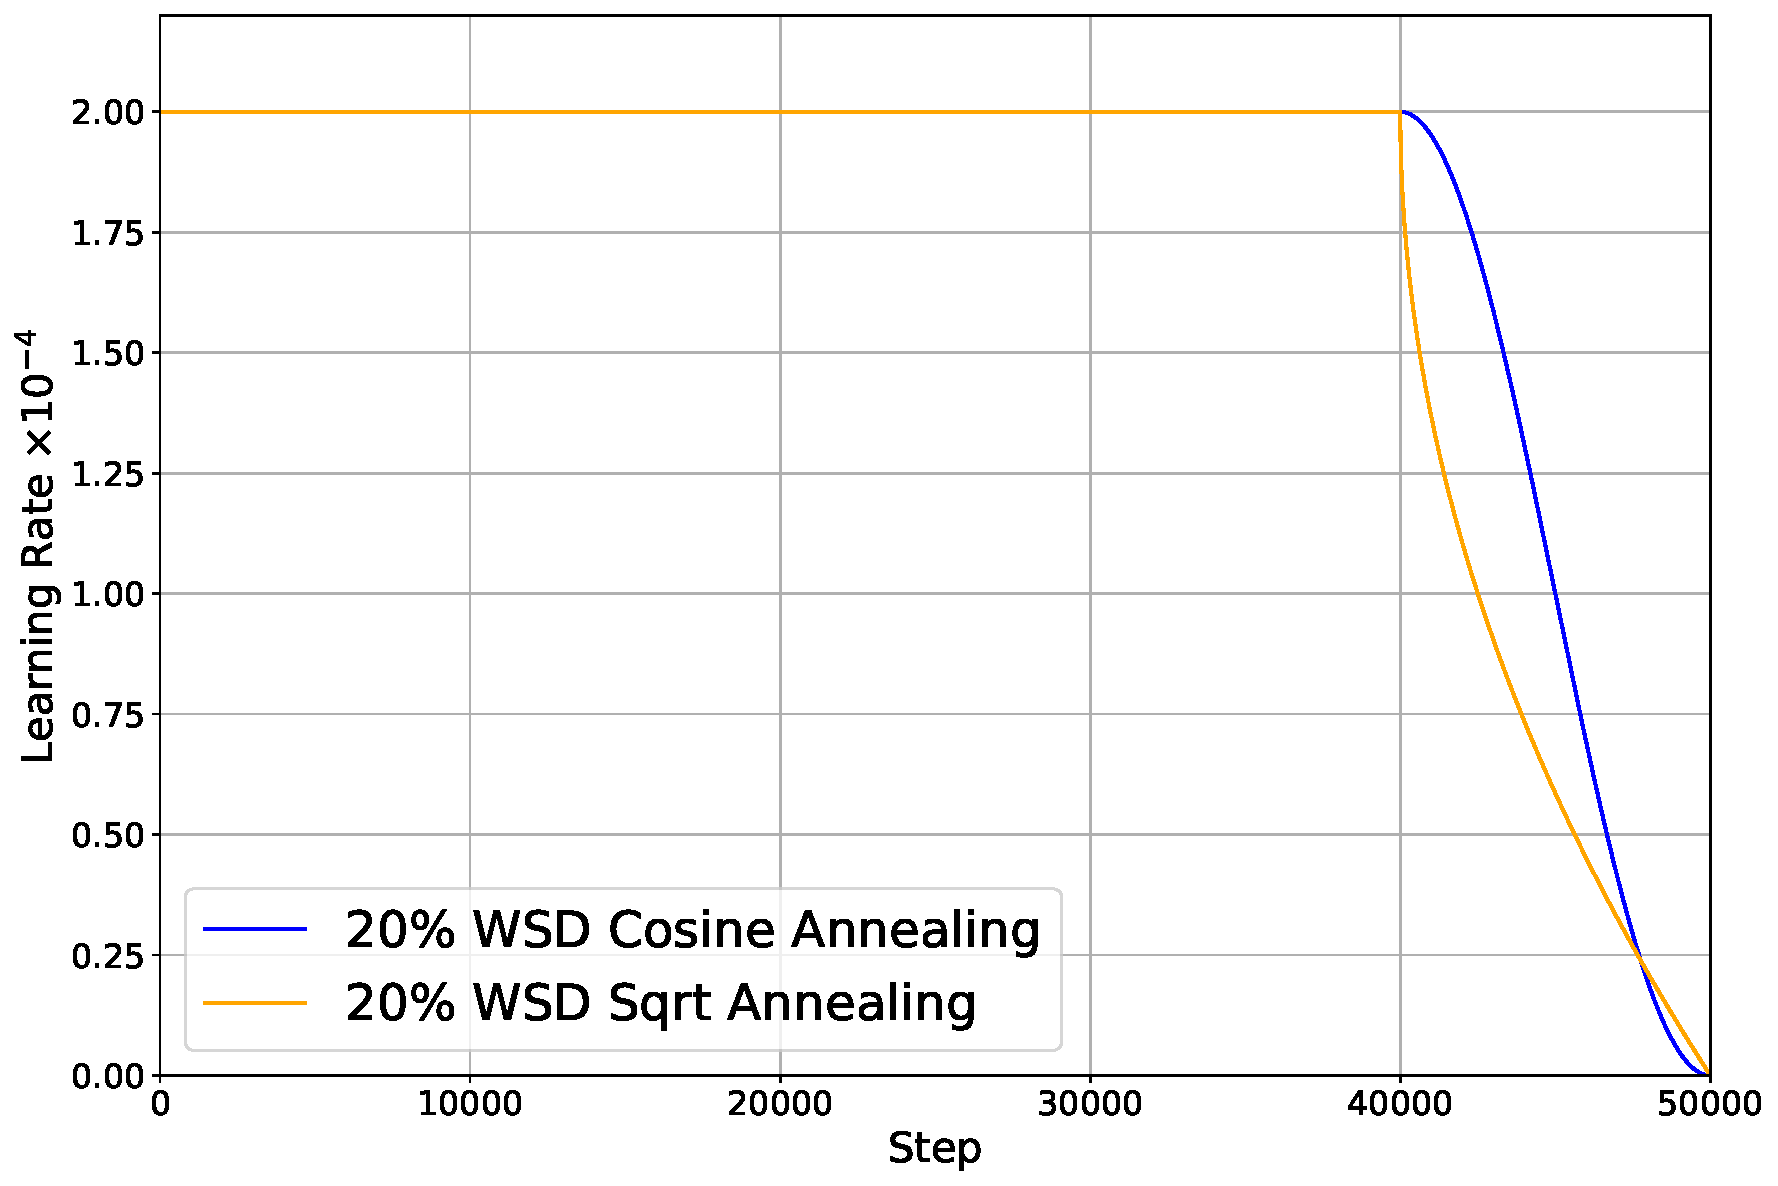
\includegraphics[width=\textwidth]{images/20_wsd.pdf}
        \caption{LR curve of WSD (20\% 1-sqrt/cosine annealing).}
    \end{subfigure}
    \hfill
    \begin{subfigure}[b]{0.48\textwidth}
        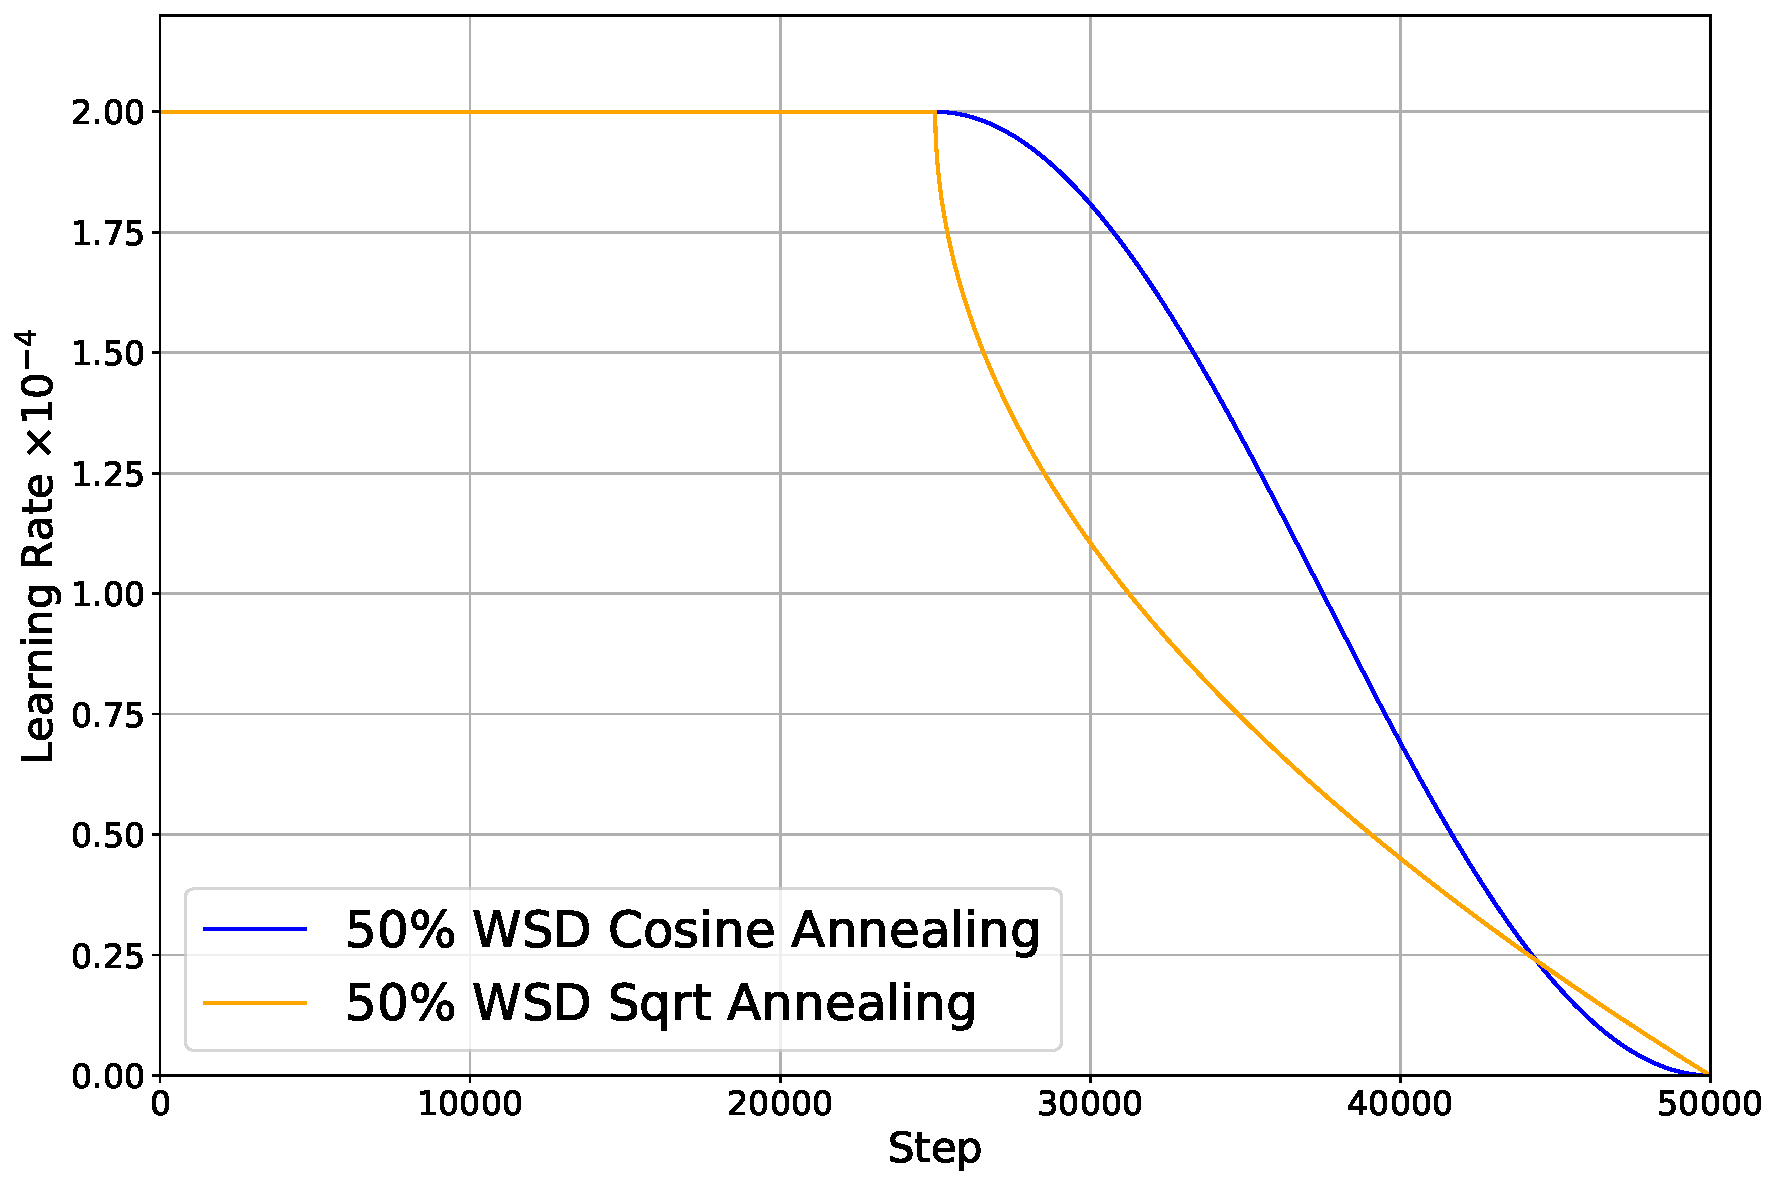
\includegraphics[width=\textwidth]{images/50_wsd.pdf}
        \caption{LR curve of WSD (50\% 1-sqrt/cosine annealing).}
    \end{subfigure}
    \caption{The learning rate curves of 20\% (left) and 50\% (right) annealing ratio in WSD LRS, with cosine and 1-sqrt annealing method.}
\label{fig:lr_1-sqrt}
\end{figure}

\citet{hu2024minicpm} proposes a warmup-stable-decay (WSD) LRS including three learning rate stages, which could help get a lower validation loss compared to the typical cosine LRS. The format is like 
\begin{equation}
\label{eq:wsd}
\begin{aligned}
WSD(s)=\begin{cases}&
\frac{s}{T_{\text {warmup}}}\eta_{max},\quad s\leq T_{\text {warmup}}\\&
\eta_{max},\quad T_{\text {warmup}}<s\leq T_{\text {stable}}\\&
\eta_{min} + f(s)\cdot(\eta_{max}-\eta_{min}),\quad T_{\text {stable}}<s\leq T_{\text {total}}
\end{cases}
\end{aligned}
\end{equation}
Where $0 \leq f(s) \leq 1$ is typically a decreasing function about step $s$, and $\eta_{max}$ is the maximal learning rate.~\citet{hägele2024scaling} consolidate the effectiveness of the WSD scheduler with numerious empirical experiments. Moreover,~\citet{hägele2024scaling} also find that using 1-sqrt annealing and a moderate
annealing ratio (e.g. 20\%) can further decrease the final loss.
\label{apx:1-sqrt}
The 1-sqrt annealing is defined as:
\begin{equation}
\begin{aligned}
&f(s)=1-\sqrt{\frac{s-T_{\text {stable }}}{T_{\text {total}} - T_{\text {stable }}}} \\ 
\end{aligned}
\end{equation}

Also, ~\citet{hägele2024scaling} mention the 1-square annealing method as a baseline, which is defined as:
\begin{equation}
\begin{aligned}
&f(s)=1-\left({\frac{s-T_{\text {stable }}}{T_{\text {total}} - T_{\text {stable }}}}\right)^2
\end{aligned}
\end{equation}

We draw the LR curve of the WSD LRS proposed by \citet{hu2024minicpm} (20\% and 50\% 1-sqrt annealing) along with the WSD LRS with a cosine annealing in Fig.~\ref{fig:lr_1-sqrt}.